\documentclass[a4paper]{article}
\usepackage[a4paper,left=3cm,right=2cm,top=2.5cm,bottom=2.5cm]{geometry}
\usepackage{palatino}
\usepackage[colorlinks=true,linkcolor=blue,citecolor=blue]{hyperref}
\usepackage{graphicx}
\usepackage{cp2021t}
\usepackage{subcaption}
\usepackage{adjustbox}
\usepackage{color}
\definecolor{red}{RGB}{255,  0,  0}
\definecolor{blue}{RGB}{0,0,255}
\def\red{\color{red}}
\def\blue{\color{blue}}
%================= local x=====================================================%
\def\getGif#1{\includegraphics[width=0.3\textwidth]{cp2021t_media/#1.png}}
\let\uk=\emph
\def\aspas#1{``#1"}
%================= lhs2tex=====================================================%
%% ODER: format ==         = "\mathrel{==}"
%% ODER: format /=         = "\neq "
%
%
\makeatletter
\@ifundefined{lhs2tex.lhs2tex.sty.read}%
  {\@namedef{lhs2tex.lhs2tex.sty.read}{}%
   \newcommand\SkipToFmtEnd{}%
   \newcommand\EndFmtInput{}%
   \long\def\SkipToFmtEnd#1\EndFmtInput{}%
  }\SkipToFmtEnd

\newcommand\ReadOnlyOnce[1]{\@ifundefined{#1}{\@namedef{#1}{}}\SkipToFmtEnd}
\usepackage{amstext}
\usepackage{amssymb}
\usepackage{stmaryrd}
\DeclareFontFamily{OT1}{cmtex}{}
\DeclareFontShape{OT1}{cmtex}{m}{n}
  {<5><6><7><8>cmtex8
   <9>cmtex9
   <10><10.95><12><14.4><17.28><20.74><24.88>cmtex10}{}
\DeclareFontShape{OT1}{cmtex}{m}{it}
  {<-> ssub * cmtt/m/it}{}
\newcommand{\texfamily}{\fontfamily{cmtex}\selectfont}
\DeclareFontShape{OT1}{cmtt}{bx}{n}
  {<5><6><7><8>cmtt8
   <9>cmbtt9
   <10><10.95><12><14.4><17.28><20.74><24.88>cmbtt10}{}
\DeclareFontShape{OT1}{cmtex}{bx}{n}
  {<-> ssub * cmtt/bx/n}{}
\newcommand{\tex}[1]{\text{\texfamily#1}}	% NEU

\newcommand{\Sp}{\hskip.33334em\relax}


\newcommand{\Conid}[1]{\mathit{#1}}
\newcommand{\Varid}[1]{\mathit{#1}}
\newcommand{\anonymous}{\kern0.06em \vbox{\hrule\@width.5em}}
\newcommand{\plus}{\mathbin{+\!\!\!+}}
\newcommand{\bind}{\mathbin{>\!\!\!>\mkern-6.7mu=}}
\newcommand{\rbind}{\mathbin{=\mkern-6.7mu<\!\!\!<}}% suggested by Neil Mitchell
\newcommand{\sequ}{\mathbin{>\!\!\!>}}
\renewcommand{\leq}{\leqslant}
\renewcommand{\geq}{\geqslant}
\usepackage{polytable}

%mathindent has to be defined
\@ifundefined{mathindent}%
  {\newdimen\mathindent\mathindent\leftmargini}%
  {}%

\def\resethooks{%
  \global\let\SaveRestoreHook\empty
  \global\let\ColumnHook\empty}
\newcommand*{\savecolumns}[1][default]%
  {\g@addto@macro\SaveRestoreHook{\savecolumns[#1]}}
\newcommand*{\restorecolumns}[1][default]%
  {\g@addto@macro\SaveRestoreHook{\restorecolumns[#1]}}
\newcommand*{\aligncolumn}[2]%
  {\g@addto@macro\ColumnHook{\column{#1}{#2}}}

\resethooks

\newcommand{\onelinecommentchars}{\quad-{}- }
\newcommand{\commentbeginchars}{\enskip\{-}
\newcommand{\commentendchars}{-\}\enskip}

\newcommand{\visiblecomments}{%
  \let\onelinecomment=\onelinecommentchars
  \let\commentbegin=\commentbeginchars
  \let\commentend=\commentendchars}

\newcommand{\invisiblecomments}{%
  \let\onelinecomment=\empty
  \let\commentbegin=\empty
  \let\commentend=\empty}

\visiblecomments

\newlength{\blanklineskip}
\setlength{\blanklineskip}{0.66084ex}

\newcommand{\hsindent}[1]{\quad}% default is fixed indentation
\let\hspre\empty
\let\hspost\empty
\newcommand{\NB}{\textbf{NB}}
\newcommand{\Todo}[1]{$\langle$\textbf{To do:}~#1$\rangle$}

\EndFmtInput
\makeatother
%
%
%
%
%
%
% This package provides two environments suitable to take the place
% of hscode, called "plainhscode" and "arrayhscode". 
%
% The plain environment surrounds each code block by vertical space,
% and it uses \abovedisplayskip and \belowdisplayskip to get spacing
% similar to formulas. Note that if these dimensions are changed,
% the spacing around displayed math formulas changes as well.
% All code is indented using \leftskip.
%
% Changed 19.08.2004 to reflect changes in colorcode. Should work with
% CodeGroup.sty.
%
\ReadOnlyOnce{polycode.fmt}%
\makeatletter

\newcommand{\hsnewpar}[1]%
  {{\parskip=0pt\parindent=0pt\par\vskip #1\noindent}}

% can be used, for instance, to redefine the code size, by setting the
% command to \small or something alike
\newcommand{\hscodestyle}{}

% The command \sethscode can be used to switch the code formatting
% behaviour by mapping the hscode environment in the subst directive
% to a new LaTeX environment.

\newcommand{\sethscode}[1]%
  {\expandafter\let\expandafter\hscode\csname #1\endcsname
   \expandafter\let\expandafter\endhscode\csname end#1\endcsname}

% "compatibility" mode restores the non-polycode.fmt layout.

\newenvironment{compathscode}%
  {\par\noindent
   \advance\leftskip\mathindent
   \hscodestyle
   \let\\=\@normalcr
   \let\hspre\(\let\hspost\)%
   \pboxed}%
  {\endpboxed\)%
   \par\noindent
   \ignorespacesafterend}

\newcommand{\compaths}{\sethscode{compathscode}}

% "plain" mode is the proposed default.
% It should now work with \centering.
% This required some changes. The old version
% is still available for reference as oldplainhscode.

\newenvironment{plainhscode}%
  {\hsnewpar\abovedisplayskip
   \advance\leftskip\mathindent
   \hscodestyle
   \let\hspre\(\let\hspost\)%
   \pboxed}%
  {\endpboxed%
   \hsnewpar\belowdisplayskip
   \ignorespacesafterend}

\newenvironment{oldplainhscode}%
  {\hsnewpar\abovedisplayskip
   \advance\leftskip\mathindent
   \hscodestyle
   \let\\=\@normalcr
   \(\pboxed}%
  {\endpboxed\)%
   \hsnewpar\belowdisplayskip
   \ignorespacesafterend}

% Here, we make plainhscode the default environment.

\newcommand{\plainhs}{\sethscode{plainhscode}}
\newcommand{\oldplainhs}{\sethscode{oldplainhscode}}
\plainhs

% The arrayhscode is like plain, but makes use of polytable's
% parray environment which disallows page breaks in code blocks.

\newenvironment{arrayhscode}%
  {\hsnewpar\abovedisplayskip
   \advance\leftskip\mathindent
   \hscodestyle
   \let\\=\@normalcr
   \(\parray}%
  {\endparray\)%
   \hsnewpar\belowdisplayskip
   \ignorespacesafterend}

\newcommand{\arrayhs}{\sethscode{arrayhscode}}

% The mathhscode environment also makes use of polytable's parray 
% environment. It is supposed to be used only inside math mode 
% (I used it to typeset the type rules in my thesis).

\newenvironment{mathhscode}%
  {\parray}{\endparray}

\newcommand{\mathhs}{\sethscode{mathhscode}}

% texths is similar to mathhs, but works in text mode.

\newenvironment{texthscode}%
  {\(\parray}{\endparray\)}

\newcommand{\texths}{\sethscode{texthscode}}

% The framed environment places code in a framed box.

\def\codeframewidth{\arrayrulewidth}
\RequirePackage{calc}

\newenvironment{framedhscode}%
  {\parskip=\abovedisplayskip\par\noindent
   \hscodestyle
   \arrayrulewidth=\codeframewidth
   \tabular{@{}|p{\linewidth-2\arraycolsep-2\arrayrulewidth-2pt}|@{}}%
   \hline\framedhslinecorrect\\{-1.5ex}%
   \let\endoflinesave=\\
   \let\\=\@normalcr
   \(\pboxed}%
  {\endpboxed\)%
   \framedhslinecorrect\endoflinesave{.5ex}\hline
   \endtabular
   \parskip=\belowdisplayskip\par\noindent
   \ignorespacesafterend}

\newcommand{\framedhslinecorrect}[2]%
  {#1[#2]}

\newcommand{\framedhs}{\sethscode{framedhscode}}

% The inlinehscode environment is an experimental environment
% that can be used to typeset displayed code inline.

\newenvironment{inlinehscode}%
  {\(\def\column##1##2{}%
   \let\>\undefined\let\<\undefined\let\\\undefined
   \newcommand\>[1][]{}\newcommand\<[1][]{}\newcommand\\[1][]{}%
   \def\fromto##1##2##3{##3}%
   \def\nextline{}}{\) }%

\newcommand{\inlinehs}{\sethscode{inlinehscode}}

% The joincode environment is a separate environment that
% can be used to surround and thereby connect multiple code
% blocks.

\newenvironment{joincode}%
  {\let\orighscode=\hscode
   \let\origendhscode=\endhscode
   \def\endhscode{\def\hscode{\endgroup\def\@currenvir{hscode}\\}\begingroup}
   %\let\SaveRestoreHook=\empty
   %\let\ColumnHook=\empty
   %\let\resethooks=\empty
   \orighscode\def\hscode{\endgroup\def\@currenvir{hscode}}}%
  {\origendhscode
   \global\let\hscode=\orighscode
   \global\let\endhscode=\origendhscode}%

\makeatother
\EndFmtInput
%
\def\ana#1{\mathopen{[\!(}#1\mathclose{)\!]}}
%%format (bin (n) (k)) = "\Big(\vcenter{\xymatrix@R=1pt{" n "\\" k "}}\Big)"


%---------------------------------------------------------------------------

\title{
       	Cálculo de Programas
\\
       	Trabalho Prático
\\
       	MiEI+LCC --- 2020/21
}

\author{
       	\dium
\\
       	Universidade do Minho
}


\date\mydate

\makeindex
\newcommand{\rn}[1]{\textcolor{red}{#1}}
\begin{document}

\maketitle

\begin{center}\large
\begin{tabular}{ll}
\textbf{Grupo} nr. & 17 
\\\hline
a91683 & Alef Pinto Keuffer 
\\
a93546 & Fernando Maria Bicalho 
\\
a88062 & Pedro Paulo Costa Pereira
\\
a91693 & Tiago André Oliveira Leite 
\end{tabular}
\end{center}

\section{Preâmbulo}

\CP\ tem como objectivo principal ensinar
a progra\-mação de computadores como uma disciplina científica. Para isso
parte-se de um repertório de \emph{combinadores} que formam uma álgebra da
programação (conjunto de leis universais e seus corolários) e usam-se esses
combinadores para construir programas \emph{composicionalmente}, isto é,
agregando programas já existentes.

Na sequência pedagógica dos planos de estudo dos dois cursos que têm
esta disciplina, opta-se pela aplicação deste método à programação
em \Haskell\ (sem prejuízo da sua aplicação a outras linguagens
funcionais). Assim, o presente trabalho prático coloca os
alunos perante problemas concretos que deverão ser implementados em
\Haskell.  Há ainda um outro objectivo: o de ensinar a documentar
programas, a validá-los e a produzir textos técnico-científicos de
qualidade.

\section{Documentação} Para cumprir de forma integrada os objectivos
enunciados acima vamos recorrer a uma técnica de programa\-ção dita
``\litp{literária}'' \cite{Kn92}, cujo princípio base é o seguinte:
%
\begin{quote}\em Um programa e a sua documentação devem coincidir.
\end{quote}
%
Por outras palavras, o código fonte e a documentação de um
programa deverão estar no mesmo ficheiro.

O ficheiro \texttt{cp2021t.pdf} que está a ler é já um exemplo de
\litp{programação literária}: foi gerado a partir do texto fonte
\texttt{cp2021t.lhs}\footnote{O suffixo `lhs' quer dizer
\emph{\lhaskell{literate Haskell}}.} que encontrará no
\MaterialPedagogico\ desta disciplina descompactando o ficheiro
\texttt{cp2021t.zip} e executando:
\begin{Verbatim}[fontsize=\small]
    $ lhs2TeX cp2021t.lhs > cp2021t.tex
    $ pdflatex cp2021t
\end{Verbatim}
em que \href{https://hackage.haskell.org/package/lhs2tex}{\texttt\LhsToTeX} é
um pre-processador que faz ``pretty printing''
de código Haskell em \Latex\ e que deve desde já instalar executando
\begin{Verbatim}[fontsize=\small]
    $ cabal install lhs2tex --lib
\end{Verbatim}
Por outro lado, o mesmo ficheiro \texttt{cp2021t.lhs} é executável e contém
o ``kit'' básico, escrito em \Haskell, para realizar o trabalho. Basta executar
\begin{Verbatim}[fontsize=\small]
    $ ghci cp2021t.lhs
\end{Verbatim}


\noindent Abra o ficheiro \texttt{cp2021t.lhs} no seu editor de texto preferido
e verifique que assim é: todo o texto que se encontra dentro do ambiente
\begin{quote}\small\tt
\text{\ttfamily \char92{}begin\char123{}code\char125{}}
\\ ... \\
\text{\ttfamily \char92{}end\char123{}code\char125{}}
\end{quote}
é seleccionado pelo \GHCi\ para ser executado.

\section{Como realizar o trabalho}
Este trabalho teórico-prático deve ser realizado por grupos de 3 (ou 4) alunos.
Os detalhes da avaliação (datas para submissão do relatório e sua defesa
oral) são os que forem publicados na \cp{página da disciplina} na \emph{internet}.

Recomenda-se uma abordagem participativa dos membros do grupo
de trabalho por forma a poderem responder às questões que serão colocadas
na \emph{defesa oral} do relatório.

Em que consiste, então, o \emph{relatório} a que se refere o parágrafo anterior?
É a edição do texto que está a ser lido, preenchendo o anexo \ref{sec:resolucao}
com as respostas. O relatório deverá conter ainda a identificação dos membros
do grupo de trabalho, no local respectivo da folha de rosto.

Para gerar o PDF integral do relatório deve-se ainda correr os comando seguintes,
que actualizam a bibliografia (com \Bibtex) e o índice remissivo (com \Makeindex),
\begin{Verbatim}[fontsize=\small]
    $ bibtex cp2021t.aux
    $ makeindex cp2021t.idx
\end{Verbatim}
e recompilar o texto como acima se indicou. Dever-se-á ainda instalar o utilitário
\QuickCheck,
que ajuda a validar programas em \Haskell\ e a biblioteca \gloss{Gloss} para
geração de gráficos 2D:
\begin{Verbatim}[fontsize=\small]
    $ cabal install QuickCheck gloss --lib
\end{Verbatim}
Para testar uma propriedade \QuickCheck~\ensuremath{\Varid{prop}}, basta invocá-la com o comando:
\begin{tabbing}\ttfamily
~~~~~\char62{}~quickCheck~prop\\
\ttfamily ~~~~~\char43{}\char43{}\char43{}~OK\char44{}~passed~100~tests\char46{}
\end{tabbing}
Pode-se ainda controlar o número de casos de teste e sua complexidade,
como o seguinte exemplo mostra:
\begin{tabbing}\ttfamily
~~~~~\char62{}~quickCheckWith~stdArgs~\char123{}~maxSuccess~\char61{}~200\char44{}~maxSize~\char61{}~10~\char125{}~prop\\
\ttfamily ~~~~~\char43{}\char43{}\char43{}~OK\char44{}~passed~200~tests\char46{}
\end{tabbing}
Qualquer programador tem, na vida real, de ler e analisar (muito!) código
escrito por outros. No anexo \ref{sec:codigo} disponibiliza-se algum
código \Haskell\ relativo aos problemas que se seguem. Esse anexo deverá
ser consultado e analisado à medida que isso for necessário.

\subsection{Stack}

O \stack{Stack} é um programa útil para criar, gerir e manter projetos em \Haskell.
Um projeto criado com o Stack possui uma estrutura de pastas muito específica:

\begin{itemize}
\item Os módulos auxiliares encontram-se na pasta \emph{src}.
\item O módulos principal encontra-se na pasta \emph{app}.
\item A lista de depêndencias externas encontra-se no ficheiro \emph{package.yaml}.
\end{itemize}

Pode aceder ao \GHCi\ utilizando o comando:
\begin{tabbing}\ttfamily
~stack~ghci
\end{tabbing}

Garanta que se encontra na pasta mais externa \textbf{do projeto}.
A primeira vez que correr este comando as depêndencias externas serão instaladas automaticamente.

Para gerar o PDF, garanta que se encontra na diretoria \emph{app}.

\Problema

Os \emph{tipos de dados algébricos} estudados ao longo desta disciplina oferecem
uma grande capacidade expressiva ao programador. Graças à sua flexibilidade,
torna-se trivial implementar \DSL s
e até mesmo \href{http://www.cse.chalmers.se/~ulfn/papers/thesis.pdf}{linguagens de programação}.

Paralelamente, um tópico bastante estudado no âmbito de \DL\
é a derivação automática de expressões matemáticas, por exemplo, de derivadas.
Duas técnicas que podem ser utilizadas para o cálculo de derivadas são:

\begin{itemize}
\item \emph{Symbolic differentiation}
\item \emph{Automatic differentiation}
\end{itemize}

\emph{Symbolic differentiation} consiste na aplicação sucessiva de transformações
(leia-se: funções) que sejam congruentes com as regras de derivação. O resultado
final será a expressão da derivada.

O leitor atento poderá notar um problema desta técnica: a expressão
inicial pode crescer de forma descontrolada, levando a um cálculo pouco eficiente.
\emph{Automatic differentiation} tenta resolver este problema,
calculando \textbf{o valor} da derivada da expressão em todos os passos.
Para tal, é necessário calcular o valor da expressão \textbf{e} o valor da sua derivada.

Vamos de seguida definir uma linguagem de expressões matemáticas simples e
implementar as duas técnicas de derivação automática.
Para isso, seja dado o seguinte tipo de dados,

\begin{hscode}\SaveRestoreHook
\column{B}{@{}>{\hspre}l<{\hspost}@{}}%
\column{12}{@{}>{\hspre}l<{\hspost}@{}}%
\column{E}{@{}>{\hspre}l<{\hspost}@{}}%
\>[B]{}\mathbf{data}\;\Conid{ExpAr}\;\Varid{a}\mathrel{=}\Conid{X}{}\<[E]%
\\
\>[B]{}\hsindent{12}{}\<[12]%
\>[12]{}\mid \Conid{N}\;\Varid{a}{}\<[E]%
\\
\>[B]{}\hsindent{12}{}\<[12]%
\>[12]{}\mid \Conid{Bin}\;\Conid{BinOp}\;(\Conid{ExpAr}\;\Varid{a})\;(\Conid{ExpAr}\;\Varid{a}){}\<[E]%
\\
\>[B]{}\hsindent{12}{}\<[12]%
\>[12]{}\mid \Conid{Un}\;\Conid{UnOp}\;(\Conid{ExpAr}\;\Varid{a}){}\<[E]%
\\
\>[B]{}\hsindent{12}{}\<[12]%
\>[12]{}\mathbf{deriving}\;(\Conid{Eq},\Conid{Show}){}\<[E]%
\ColumnHook
\end{hscode}\resethooks

\noindent
onde \ensuremath{\Conid{BinOp}} e \ensuremath{\Conid{UnOp}} representam operações binárias e unárias, respectivamente:

\begin{hscode}\SaveRestoreHook
\column{B}{@{}>{\hspre}l<{\hspost}@{}}%
\column{11}{@{}>{\hspre}l<{\hspost}@{}}%
\column{12}{@{}>{\hspre}l<{\hspost}@{}}%
\column{E}{@{}>{\hspre}l<{\hspost}@{}}%
\>[B]{}\mathbf{data}\;\Conid{BinOp}\mathrel{=}\Conid{Sum}{}\<[E]%
\\
\>[B]{}\hsindent{12}{}\<[12]%
\>[12]{}\mid \Conid{Product}{}\<[E]%
\\
\>[B]{}\hsindent{12}{}\<[12]%
\>[12]{}\mathbf{deriving}\;(\Conid{Eq},\Conid{Show}){}\<[E]%
\\[\blanklineskip]%
\>[B]{}\mathbf{data}\;\Conid{UnOp}\mathrel{=}\Conid{Negate}{}\<[E]%
\\
\>[B]{}\hsindent{11}{}\<[11]%
\>[11]{}\mid \Conid{E}{}\<[E]%
\\
\>[B]{}\hsindent{11}{}\<[11]%
\>[11]{}\mathbf{deriving}\;(\Conid{Eq},\Conid{Show}){}\<[E]%
\ColumnHook
\end{hscode}\resethooks

\noindent
O construtor \ensuremath{\Conid{E}} simboliza o exponencial de base $e$.

Assim, cada expressão pode ser uma variável, um número, uma operação binária
aplicada às devidas expressões, ou uma operação unária aplicada a uma expressão.
Por exemplo,
\begin{hscode}\SaveRestoreHook
\column{B}{@{}>{\hspre}l<{\hspost}@{}}%
\column{E}{@{}>{\hspre}l<{\hspost}@{}}%
\>[B]{}\Conid{Bin}\;\Conid{Sum}\;\Conid{X}\;(\Conid{N}\;\mathrm{10}){}\<[E]%
\ColumnHook
\end{hscode}\resethooks
designa \ensuremath{\Varid{x}\mathbin{+}\mathrm{10}} na notação matemática habitual.

\begin{enumerate}
\item A definição das funções \ensuremath{\Varid{inExpAr}} e \ensuremath{\Varid{baseExpAr}} para este tipo é a seguinte:
\begin{hscode}\SaveRestoreHook
\column{B}{@{}>{\hspre}l<{\hspost}@{}}%
\column{3}{@{}>{\hspre}l<{\hspost}@{}}%
\column{11}{@{}>{\hspre}l<{\hspost}@{}}%
\column{E}{@{}>{\hspre}l<{\hspost}@{}}%
\>[B]{}\Varid{inExpAr}\mathrel{=}\alt{\underline{\Conid{X}}}{\Varid{num\char95 ops}}\;\mathbf{where}{}\<[E]%
\\
\>[B]{}\hsindent{3}{}\<[3]%
\>[3]{}\Varid{num\char95 ops}\mathrel{=}\alt{\Conid{N}}{\Varid{ops}}{}\<[E]%
\\
\>[B]{}\hsindent{3}{}\<[3]%
\>[3]{}\Varid{ops}{}\<[11]%
\>[11]{}\mathrel{=}\alt{\Varid{bin}}{\uncurry{\Conid{Un}}}{}\<[E]%
\\
\>[B]{}\hsindent{3}{}\<[3]%
\>[3]{}\Varid{bin}\;(\Varid{op},(\Varid{a},\Varid{b}))\mathrel{=}\Conid{Bin}\;\Varid{op}\;\Varid{a}\;\Varid{b}{}\<[E]%
\\[\blanklineskip]%
\>[B]{}\Varid{baseExpAr}\;\Varid{f}\;\Varid{g}\;\Varid{h}\;\Varid{j}\;\Varid{k}\;\Varid{l}\;\Varid{z}\mathrel{=}\Varid{f}+(\Varid{g}+(\Varid{h}\times(\Varid{j}\times\Varid{k})+\Varid{l}\times\Varid{z})){}\<[E]%
\ColumnHook
\end{hscode}\resethooks

  Defina as funções \ensuremath{\Varid{outExpAr}} e \ensuremath{\Varid{recExpAr}},
  e teste as propriedades que se seguem.
  \begin{propriedade}
    \ensuremath{\Varid{inExpAr}} e \ensuremath{\Varid{outExpAr}} são testemunhas de um isomorfismo,
    isto é,
    \ensuremath{\Varid{inExpAr}\comp \Varid{outExpAr}\mathrel{=}\Varid{id}} e \ensuremath{\Varid{outExpAr}\comp \Varid{idExpAr}\mathrel{=}\Varid{id}}:
\begin{hscode}\SaveRestoreHook
\column{B}{@{}>{\hspre}l<{\hspost}@{}}%
\column{E}{@{}>{\hspre}l<{\hspost}@{}}%
\>[B]{}\Varid{prop\char95 in\char95 out\char95 idExpAr}\mathbin{::}(\Conid{Eq}\;\Varid{a})\Rightarrow \Conid{ExpAr}\;\Varid{a}\to \Conid{Bool}{}\<[E]%
\\
\>[B]{}\Varid{prop\char95 in\char95 out\char95 idExpAr}\mathrel{=}\Varid{inExpAr}\comp \Varid{outExpAr}\equiv\Varid{id}{}\<[E]%
\\[\blanklineskip]%
\>[B]{}\Varid{prop\char95 out\char95 in\char95 idExpAr}\mathbin{::}(\Conid{Eq}\;\Varid{a})\Rightarrow \Conid{OutExpAr}\;\Varid{a}\to \Conid{Bool}{}\<[E]%
\\
\>[B]{}\Varid{prop\char95 out\char95 in\char95 idExpAr}\mathrel{=}\Varid{outExpAr}\comp \Varid{inExpAr}\equiv\Varid{id}{}\<[E]%
\ColumnHook
\end{hscode}\resethooks
    \end{propriedade}

  \item Dada uma expressão aritmética e um escalar para substituir o \ensuremath{\Conid{X}},
	a função

\begin{quote}
      \ensuremath{\Varid{eval\char95 exp}\mathbin{::}\Conid{Floating}\;\Varid{a}\Rightarrow \Varid{a}\to (\Conid{ExpAr}\;\Varid{a})\to \Varid{a}}
\end{quote}

\noindent calcula o resultado da expressão. Na página \pageref{pg:P1}
    esta função está expressa como um catamorfismo. Defina o respectivo gene
    e, de seguida, teste as propriedades:
    \begin{propriedade}
       A função \ensuremath{\Varid{eval\char95 exp}} respeita os elementos neutros das operações.
\begin{hscode}\SaveRestoreHook
\column{B}{@{}>{\hspre}l<{\hspost}@{}}%
\column{3}{@{}>{\hspre}l<{\hspost}@{}}%
\column{E}{@{}>{\hspre}l<{\hspost}@{}}%
\>[B]{}\Varid{prop\char95 sum\char95 idr}\mathbin{::}(\Conid{Floating}\;\Varid{a},\Conid{Real}\;\Varid{a})\Rightarrow \Varid{a}\to \Conid{ExpAr}\;\Varid{a}\to \Conid{Bool}{}\<[E]%
\\
\>[B]{}\Varid{prop\char95 sum\char95 idr}\;\Varid{a}\;\Varid{exp}\mathrel{=}\Varid{eval\char95 exp}\;\Varid{a}\;\Varid{exp}\mathbin{\stackrel{\mathrm{?}}{=}}\Varid{sum\char95 idr}\;\mathbf{where}{}\<[E]%
\\
\>[B]{}\hsindent{3}{}\<[3]%
\>[3]{}\Varid{sum\char95 idr}\mathrel{=}\Varid{eval\char95 exp}\;\Varid{a}\;(\Conid{Bin}\;\Conid{Sum}\;\Varid{exp}\;(\Conid{N}\;\mathrm{0})){}\<[E]%
\\[\blanklineskip]%
\>[B]{}\Varid{prop\char95 sum\char95 idl}\mathbin{::}(\Conid{Floating}\;\Varid{a},\Conid{Real}\;\Varid{a})\Rightarrow \Varid{a}\to \Conid{ExpAr}\;\Varid{a}\to \Conid{Bool}{}\<[E]%
\\
\>[B]{}\Varid{prop\char95 sum\char95 idl}\;\Varid{a}\;\Varid{exp}\mathrel{=}\Varid{eval\char95 exp}\;\Varid{a}\;\Varid{exp}\mathbin{\stackrel{\mathrm{?}}{=}}\Varid{sum\char95 idl}\;\mathbf{where}{}\<[E]%
\\
\>[B]{}\hsindent{3}{}\<[3]%
\>[3]{}\Varid{sum\char95 idl}\mathrel{=}\Varid{eval\char95 exp}\;\Varid{a}\;(\Conid{Bin}\;\Conid{Sum}\;(\Conid{N}\;\mathrm{0})\;\Varid{exp}){}\<[E]%
\\[\blanklineskip]%
\>[B]{}\Varid{prop\char95 product\char95 idr}\mathbin{::}(\Conid{Floating}\;\Varid{a},\Conid{Real}\;\Varid{a})\Rightarrow \Varid{a}\to \Conid{ExpAr}\;\Varid{a}\to \Conid{Bool}{}\<[E]%
\\
\>[B]{}\Varid{prop\char95 product\char95 idr}\;\Varid{a}\;\Varid{exp}\mathrel{=}\Varid{eval\char95 exp}\;\Varid{a}\;\Varid{exp}\mathbin{\stackrel{\mathrm{?}}{=}}\Varid{prod\char95 idr}\;\mathbf{where}{}\<[E]%
\\
\>[B]{}\hsindent{3}{}\<[3]%
\>[3]{}\Varid{prod\char95 idr}\mathrel{=}\Varid{eval\char95 exp}\;\Varid{a}\;(\Conid{Bin}\;\Conid{Product}\;\Varid{exp}\;(\Conid{N}\;\mathrm{1})){}\<[E]%
\\[\blanklineskip]%
\>[B]{}\Varid{prop\char95 product\char95 idl}\mathbin{::}(\Conid{Floating}\;\Varid{a},\Conid{Real}\;\Varid{a})\Rightarrow \Varid{a}\to \Conid{ExpAr}\;\Varid{a}\to \Conid{Bool}{}\<[E]%
\\
\>[B]{}\Varid{prop\char95 product\char95 idl}\;\Varid{a}\;\Varid{exp}\mathrel{=}\Varid{eval\char95 exp}\;\Varid{a}\;\Varid{exp}\mathbin{\stackrel{\mathrm{?}}{=}}\Varid{prod\char95 idl}\;\mathbf{where}{}\<[E]%
\\
\>[B]{}\hsindent{3}{}\<[3]%
\>[3]{}\Varid{prod\char95 idl}\mathrel{=}\Varid{eval\char95 exp}\;\Varid{a}\;(\Conid{Bin}\;\Conid{Product}\;(\Conid{N}\;\mathrm{1})\;\Varid{exp}){}\<[E]%
\\[\blanklineskip]%
\>[B]{}\Varid{prop\char95 e\char95 id}\mathbin{::}(\Conid{Floating}\;\Varid{a},\Conid{Real}\;\Varid{a})\Rightarrow \Varid{a}\to \Conid{Bool}{}\<[E]%
\\
\>[B]{}\Varid{prop\char95 e\char95 id}\;\Varid{a}\mathrel{=}\Varid{eval\char95 exp}\;\Varid{a}\;(\Conid{Un}\;\Conid{E}\;(\Conid{N}\;\mathrm{1}))\equiv \Varid{expd}\;\mathrm{1}{}\<[E]%
\\[\blanklineskip]%
\>[B]{}\Varid{prop\char95 negate\char95 id}\mathbin{::}(\Conid{Floating}\;\Varid{a},\Conid{Real}\;\Varid{a})\Rightarrow \Varid{a}\to \Conid{Bool}{}\<[E]%
\\
\>[B]{}\Varid{prop\char95 negate\char95 id}\;\Varid{a}\mathrel{=}\Varid{eval\char95 exp}\;\Varid{a}\;(\Conid{Un}\;\Conid{Negate}\;(\Conid{N}\;\mathrm{0}))\equiv \mathrm{0}{}\<[E]%
\ColumnHook
\end{hscode}\resethooks
    \end{propriedade}
    \begin{propriedade}
      Negar duas vezes uma expressão tem o mesmo valor que não fazer nada.
\begin{hscode}\SaveRestoreHook
\column{B}{@{}>{\hspre}l<{\hspost}@{}}%
\column{E}{@{}>{\hspre}l<{\hspost}@{}}%
\>[B]{}\Varid{prop\char95 double\char95 negate}\mathbin{::}(\Conid{Floating}\;\Varid{a},\Conid{Real}\;\Varid{a})\Rightarrow \Varid{a}\to \Conid{ExpAr}\;\Varid{a}\to \Conid{Bool}{}\<[E]%
\\
\>[B]{}\Varid{prop\char95 double\char95 negate}\;\Varid{a}\;\Varid{exp}\mathrel{=}\Varid{eval\char95 exp}\;\Varid{a}\;\Varid{exp}\mathbin{\stackrel{\mathrm{?}}{=}}\Varid{eval\char95 exp}\;\Varid{a}\;(\Conid{Un}\;\Conid{Negate}\;(\Conid{Un}\;\Conid{Negate}\;\Varid{exp})){}\<[E]%
\ColumnHook
\end{hscode}\resethooks
    \end{propriedade}

  \item É possível otimizar o cálculo do valor de uma expressão aritmética tirando proveito
  dos elementos absorventes de cada operação. Implemente os genes da função
\begin{hscode}\SaveRestoreHook
\column{B}{@{}>{\hspre}l<{\hspost}@{}}%
\column{7}{@{}>{\hspre}l<{\hspost}@{}}%
\column{E}{@{}>{\hspre}l<{\hspost}@{}}%
\>[7]{}\Varid{optmize\char95 eval}\mathbin{::}(\Conid{Floating}\;\Varid{a},\Conid{Eq}\;\Varid{a})\Rightarrow \Varid{a}\to (\Conid{ExpAr}\;\Varid{a})\to \Varid{a}{}\<[E]%
\ColumnHook
\end{hscode}\resethooks
  que se encontra na página \pageref{pg:P1} expressa como um hilomorfismo\footnote{Qual é a vantagem de implementar a função \ensuremath{\Varid{optimize\char95 eval}} utilizando um hilomorfismo em vez de utilizar um catamorfismo com um gene "inteligente"?}
  e teste as propriedades:

    \begin{propriedade}
      A função \ensuremath{\Varid{optimize\char95 eval}} respeita a semântica da função \ensuremath{\Varid{eval}}.
\begin{hscode}\SaveRestoreHook
\column{B}{@{}>{\hspre}l<{\hspost}@{}}%
\column{E}{@{}>{\hspre}l<{\hspost}@{}}%
\>[B]{}\Varid{prop\char95 optimize\char95 respects\char95 semantics}\mathbin{::}(\Conid{Floating}\;\Varid{a},\Conid{Real}\;\Varid{a})\Rightarrow \Varid{a}\to \Conid{ExpAr}\;\Varid{a}\to \Conid{Bool}{}\<[E]%
\\
\>[B]{}\Varid{prop\char95 optimize\char95 respects\char95 semantics}\;\Varid{a}\;\Varid{exp}\mathrel{=}\Varid{eval\char95 exp}\;\Varid{a}\;\Varid{exp}\mathbin{\stackrel{\mathrm{?}}{=}}\Varid{optmize\char95 eval}\;\Varid{a}\;\Varid{exp}{}\<[E]%
\ColumnHook
\end{hscode}\resethooks
    \end{propriedade}


\item Para calcular a derivada de uma expressão, é necessário aplicar transformações
à expressão original que respeitem as regras das derivadas:\footnote{%
	Apesar da adição e multiplicação gozarem da propriedade comutativa,
	há que ter em atenção a ordem das operações por causa dos testes.}

\begin{itemize}
  \item Regra da soma:
\begin{eqnarray*}
	\frac{d}{dx}(f(x)+g(x))=\frac{d}{dx}(f(x))+\frac{d}{dx}(g(x))
\end{eqnarray*}
  \item Regra do produto:
\begin{eqnarray*}
	\frac{d}{dx}(f(x)g(x))=f(x)\cdot \frac{d}{dx}(g(x))+\frac{d}{dx}(f(x))\cdot g(x)
\end{eqnarray*}
\end{itemize}

  Defina o gene do catamorfismo que ocorre na função
    \begin{quote}
      \ensuremath{\Varid{sd}\mathbin{::}\Conid{Floating}\;\Varid{a}\Rightarrow \Conid{ExpAr}\;\Varid{a}\to \Conid{ExpAr}\;\Varid{a}}
    \end{quote}
  que, dada uma expressão aritmética, calcula a sua derivada.
  Testes a fazer, de seguida:
    \begin{propriedade}
       A função \ensuremath{\Varid{sd}} respeita as regras de derivação.
\begin{hscode}\SaveRestoreHook
\column{B}{@{}>{\hspre}l<{\hspost}@{}}%
\column{3}{@{}>{\hspre}l<{\hspost}@{}}%
\column{E}{@{}>{\hspre}l<{\hspost}@{}}%
\>[B]{}\Varid{prop\char95 const\char95 rule}\mathbin{::}(\Conid{Real}\;\Varid{a},\Conid{Floating}\;\Varid{a})\Rightarrow \Varid{a}\to \Conid{Bool}{}\<[E]%
\\
\>[B]{}\Varid{prop\char95 const\char95 rule}\;\Varid{a}\mathrel{=}\Varid{sd}\;(\Conid{N}\;\Varid{a})\equiv \Conid{N}\;\mathrm{0}{}\<[E]%
\\[\blanklineskip]%
\>[B]{}\Varid{prop\char95 var\char95 rule}\mathbin{::}\Conid{Bool}{}\<[E]%
\\
\>[B]{}\Varid{prop\char95 var\char95 rule}\mathrel{=}\Varid{sd}\;\Conid{X}\equiv \Conid{N}\;\mathrm{1}{}\<[E]%
\\[\blanklineskip]%
\>[B]{}\Varid{prop\char95 sum\char95 rule}\mathbin{::}(\Conid{Real}\;\Varid{a},\Conid{Floating}\;\Varid{a})\Rightarrow \Conid{ExpAr}\;\Varid{a}\to \Conid{ExpAr}\;\Varid{a}\to \Conid{Bool}{}\<[E]%
\\
\>[B]{}\Varid{prop\char95 sum\char95 rule}\;\Varid{exp1}\;\Varid{exp2}\mathrel{=}\Varid{sd}\;(\Conid{Bin}\;\Conid{Sum}\;\Varid{exp1}\;\Varid{exp2})\equiv \Varid{sum\char95 rule}\;\mathbf{where}{}\<[E]%
\\
\>[B]{}\hsindent{3}{}\<[3]%
\>[3]{}\Varid{sum\char95 rule}\mathrel{=}\Conid{Bin}\;\Conid{Sum}\;(\Varid{sd}\;\Varid{exp1})\;(\Varid{sd}\;\Varid{exp2}){}\<[E]%
\\[\blanklineskip]%
\>[B]{}\Varid{prop\char95 product\char95 rule}\mathbin{::}(\Conid{Real}\;\Varid{a},\Conid{Floating}\;\Varid{a})\Rightarrow \Conid{ExpAr}\;\Varid{a}\to \Conid{ExpAr}\;\Varid{a}\to \Conid{Bool}{}\<[E]%
\\
\>[B]{}\Varid{prop\char95 product\char95 rule}\;\Varid{exp1}\;\Varid{exp2}\mathrel{=}\Varid{sd}\;(\Conid{Bin}\;\Conid{Product}\;\Varid{exp1}\;\Varid{exp2})\equiv \Varid{prod\char95 rule}\;\mathbf{where}{}\<[E]%
\\
\>[B]{}\hsindent{3}{}\<[3]%
\>[3]{}\Varid{prod\char95 rule}\mathrel{=}\Conid{Bin}\;\Conid{Sum}\;(\Conid{Bin}\;\Conid{Product}\;\Varid{exp1}\;(\Varid{sd}\;\Varid{exp2}))\;(\Conid{Bin}\;\Conid{Product}\;(\Varid{sd}\;\Varid{exp1})\;\Varid{exp2}){}\<[E]%
\\[\blanklineskip]%
\>[B]{}\Varid{prop\char95 e\char95 rule}\mathbin{::}(\Conid{Real}\;\Varid{a},\Conid{Floating}\;\Varid{a})\Rightarrow \Conid{ExpAr}\;\Varid{a}\to \Conid{Bool}{}\<[E]%
\\
\>[B]{}\Varid{prop\char95 e\char95 rule}\;\Varid{exp}\mathrel{=}\Varid{sd}\;(\Conid{Un}\;\Conid{E}\;\Varid{exp})\equiv \Conid{Bin}\;\Conid{Product}\;(\Conid{Un}\;\Conid{E}\;\Varid{exp})\;(\Varid{sd}\;\Varid{exp}){}\<[E]%
\\[\blanklineskip]%
\>[B]{}\Varid{prop\char95 negate\char95 rule}\mathbin{::}(\Conid{Real}\;\Varid{a},\Conid{Floating}\;\Varid{a})\Rightarrow \Conid{ExpAr}\;\Varid{a}\to \Conid{Bool}{}\<[E]%
\\
\>[B]{}\Varid{prop\char95 negate\char95 rule}\;\Varid{exp}\mathrel{=}\Varid{sd}\;(\Conid{Un}\;\Conid{Negate}\;\Varid{exp})\equiv \Conid{Un}\;\Conid{Negate}\;(\Varid{sd}\;\Varid{exp}){}\<[E]%
\ColumnHook
\end{hscode}\resethooks
    \end{propriedade}

\item Como foi visto, \emph{Symbolic differentiation} não é a técnica
mais eficaz para o cálculo do valor da derivada de uma expressão.
\emph{Automatic differentiation} resolve este problema cálculando o valor
da derivada em vez de manipular a expressão original.

  Defina o gene do catamorfismo que ocorre na função
    \begin{hscode}\SaveRestoreHook
\column{B}{@{}>{\hspre}l<{\hspost}@{}}%
\column{5}{@{}>{\hspre}l<{\hspost}@{}}%
\column{E}{@{}>{\hspre}l<{\hspost}@{}}%
\>[5]{}\Varid{ad}\mathbin{::}\Conid{Floating}\;\Varid{a}\Rightarrow \Varid{a}\to \Conid{ExpAr}\;\Varid{a}\to \Varid{a}{}\<[E]%
\ColumnHook
\end{hscode}\resethooks
  que, dada uma expressão aritmética e um ponto,
  calcula o valor da sua derivada nesse ponto,
  sem transformar manipular a expressão original.
  Testes a fazer, de seguida:

    \begin{propriedade}
       Calcular o valor da derivada num ponto \ensuremath{\Varid{r}} via \ensuremath{\Varid{ad}} é equivalente a calcular a derivada da expressão e avalia-la no ponto \ensuremath{\Varid{r}}.
\begin{hscode}\SaveRestoreHook
\column{B}{@{}>{\hspre}l<{\hspost}@{}}%
\column{E}{@{}>{\hspre}l<{\hspost}@{}}%
\>[B]{}\Varid{prop\char95 congruent}\mathbin{::}(\Conid{Floating}\;\Varid{a},\Conid{Real}\;\Varid{a})\Rightarrow \Varid{a}\to \Conid{ExpAr}\;\Varid{a}\to \Conid{Bool}{}\<[E]%
\\
\>[B]{}\Varid{prop\char95 congruent}\;\Varid{a}\;\Varid{exp}\mathrel{=}\Varid{ad}\;\Varid{a}\;\Varid{exp}\mathbin{\stackrel{\mathrm{?}}{=}}\Varid{eval\char95 exp}\;\Varid{a}\;(\Varid{sd}\;\Varid{exp}){}\<[E]%
\ColumnHook
\end{hscode}\resethooks
    \end{propriedade}
\end{enumerate}

\Problema

Nesta disciplina estudou-se como fazer \pd{programação dinâmica} por cálculo,
recorrendo à lei de recursividade mútua.\footnote{Lei (\ref{eq:fokkinga})
em \cite{Ol18}, página \pageref{eq:fokkinga}.}

Para o caso de funções sobre os números naturais (\ensuremath{\N_0}, com functor \ensuremath{\fun F \;\Conid{X}\mathrel{=}\mathrm{1}\mathbin{+}\Conid{X}}) é fácil derivar-se da lei que foi estudada uma
	\emph{regra de algibeira}
	\label{pg:regra}
que se pode ensinar a programadores que não tenham estudado
\cp{Cálculo de Programas}. Apresenta-se de seguida essa regra, tomando como exemplo o
cálculo do ciclo-\textsf{for} que implementa a função de Fibonacci, recordar
o sistema
\begin{hscode}\SaveRestoreHook
\column{B}{@{}>{\hspre}l<{\hspost}@{}}%
\column{E}{@{}>{\hspre}l<{\hspost}@{}}%
\>[B]{}\Varid{fib}\;\mathrm{0}\mathrel{=}\mathrm{1}{}\<[E]%
\\
\>[B]{}\Varid{fib}\;(\Varid{n}\mathbin{+}\mathrm{1})\mathrel{=}\Varid{f}\;\Varid{n}{}\<[E]%
\\[\blanklineskip]%
\>[B]{}\Varid{f}\;\mathrm{0}\mathrel{=}\mathrm{1}{}\<[E]%
\\
\>[B]{}\Varid{f}\;(\Varid{n}\mathbin{+}\mathrm{1})\mathrel{=}\Varid{fib}\;\Varid{n}\mathbin{+}\Varid{f}\;\Varid{n}{}\<[E]%
\ColumnHook
\end{hscode}\resethooks
Obter-se-á de imediato
\begin{hscode}\SaveRestoreHook
\column{B}{@{}>{\hspre}l<{\hspost}@{}}%
\column{4}{@{}>{\hspre}l<{\hspost}@{}}%
\column{E}{@{}>{\hspre}l<{\hspost}@{}}%
\>[B]{}\Varid{fib'}\mathrel{=}\p1\comp \for{\Varid{loop}}\ {\Varid{init}}\;\mathbf{where}{}\<[E]%
\\
\>[B]{}\hsindent{4}{}\<[4]%
\>[4]{}\Varid{loop}\;(\Varid{fib},\Varid{f})\mathrel{=}(\Varid{f},\Varid{fib}\mathbin{+}\Varid{f}){}\<[E]%
\\
\>[B]{}\hsindent{4}{}\<[4]%
\>[4]{}\Varid{init}\mathrel{=}(\mathrm{1},\mathrm{1}){}\<[E]%
\ColumnHook
\end{hscode}\resethooks
usando as regras seguintes:
\begin{itemize}
\item	O corpo do ciclo \ensuremath{\Varid{loop}} terá tantos argumentos quanto o número de funções mutuamente recursivas.
\item	Para as variáveis escolhem-se os próprios nomes das funções, pela ordem
que se achar conveniente.\footnote{Podem obviamente usar-se outros símbolos, mas numa primeira leitura
dá jeito usarem-se tais nomes.}
\item	Para os resultados vão-se buscar as expressões respectivas, retirando a variável \ensuremath{\Varid{n}}.
\item	Em \ensuremath{\Varid{init}} coleccionam-se os resultados dos casos de base das funções, pela mesma ordem.
\end{itemize}
Mais um exemplo, envolvendo polinómios do segundo grau $ax^2 + b x + c$ em \ensuremath{\N_0}.
Seguindo o método estudado nas aulas\footnote{Secção 3.17 de \cite{Ol18} e tópico
\href{https://www4.di.uminho.pt/~jno/media/cp/}{Recursividade mútua} nos vídeos das aulas teóricas.},
de $f\ x = a x^2 + b x + c$ derivam-se duas funções mutuamente recursivas:
\begin{hscode}\SaveRestoreHook
\column{B}{@{}>{\hspre}l<{\hspost}@{}}%
\column{E}{@{}>{\hspre}l<{\hspost}@{}}%
\>[B]{}\Varid{f}\;\mathrm{0}\mathrel{=}\Varid{c}{}\<[E]%
\\
\>[B]{}\Varid{f}\;(\Varid{n}\mathbin{+}\mathrm{1})\mathrel{=}\Varid{f}\;\Varid{n}\mathbin{+}\Varid{k}\;\Varid{n}{}\<[E]%
\\[\blanklineskip]%
\>[B]{}\Varid{k}\;\mathrm{0}\mathrel{=}\Varid{a}\mathbin{+}\Varid{b}{}\<[E]%
\\
\>[B]{}\Varid{k}\;(\Varid{n}\mathbin{+}\mathrm{1})\mathrel{=}\Varid{k}\;\Varid{n}\mathbin{+}\mathrm{2}\;\Varid{a}{}\<[E]%
\ColumnHook
\end{hscode}\resethooks
Seguindo a regra acima, calcula-se de imediato a seguinte implementação, em Haskell:
\begin{hscode}\SaveRestoreHook
\column{B}{@{}>{\hspre}l<{\hspost}@{}}%
\column{3}{@{}>{\hspre}l<{\hspost}@{}}%
\column{E}{@{}>{\hspre}l<{\hspost}@{}}%
\>[B]{}\Varid{f'}\;\Varid{a}\;\Varid{b}\;\Varid{c}\mathrel{=}\p1\comp \for{\Varid{loop}}\ {\Varid{init}}\;\mathbf{where}{}\<[E]%
\\
\>[B]{}\hsindent{3}{}\<[3]%
\>[3]{}\Varid{loop}\;(\Varid{f},\Varid{k})\mathrel{=}(\Varid{f}\mathbin{+}\Varid{k},\Varid{k}\mathbin{+}\mathrm{2}\mathbin{*}\Varid{a}){}\<[E]%
\\
\>[B]{}\hsindent{3}{}\<[3]%
\>[3]{}\Varid{init}\mathrel{=}(\Varid{c},\Varid{a}\mathbin{+}\Varid{b}){}\<[E]%
\ColumnHook
\end{hscode}\resethooks
O que se pede então, nesta pergunta?
Dada a fórmula que dá o \ensuremath{\Varid{n}}-ésimo \catalan{número de Catalan},
\begin{eqnarray}
	C_n = \frac{(2n)!}{(n+1)! (n!) }
	\label{eq:cat}
\end{eqnarray}
derivar uma implementação de $C_n$ que não calcule factoriais nenhuns.
Isto é, derivar um ciclo-\textsf{for}
\begin{hscode}\SaveRestoreHook
\column{B}{@{}>{\hspre}l<{\hspost}@{}}%
\column{E}{@{}>{\hspre}l<{\hspost}@{}}%
\>[B]{}\Varid{cat}\mathrel{=}\cdots \comp \for{\Varid{loop}}\ {\Varid{init}}\;\mathbf{where}\;\cdots {}\<[E]%
\ColumnHook
\end{hscode}\resethooks
que implemente esta função.

\begin{propriedade}
A função proposta coincidem com a definição dada:
\begin{hscode}\SaveRestoreHook
\column{B}{@{}>{\hspre}l<{\hspost}@{}}%
\column{33}{@{}>{\hspre}l<{\hspost}@{}}%
\column{E}{@{}>{\hspre}l<{\hspost}@{}}%
\>[B]{}\Varid{prop\char95 cat}\mathrel{=}(\geq \mathrm{0})\Rightarrow(\Varid{catdef}{}\<[33]%
\>[33]{}\equiv\Varid{cat}){}\<[E]%
\ColumnHook
\end{hscode}\resethooks
\end{propriedade}
%
\textbf{Sugestão}: Começar por estudar muito bem o processo de cálculo dado
no anexo \ref{sec:recmul} para o problema (semelhante) da função exponencial.


\Problema

As \bezier{curvas de Bézier}, designação dada em honra ao engenheiro
\href{https://en.wikipedia.org/wiki/Pierre_B%C3%A9zier}{Pierre Bézier},
são curvas ubíquas na área de computação gráfica, animação e modelação.
Uma curva de Bézier é uma curva paramétrica, definida por um conjunto
$\{P_0,...,P_N\}$ de pontos de controlo, onde $N$ é a ordem da curva.

\begin{figure}[h!]
  \centering
  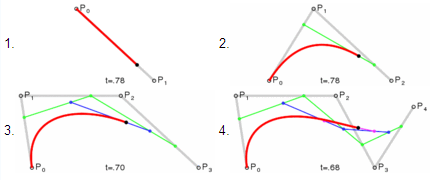
\includegraphics[width=0.8\textwidth]{cp2021t_media/Bezier_curves.png}
  \caption{Exemplos de curvas de Bézier retirados da \bezier{ Wikipedia}.}
\end{figure}

O algoritmo de \emph{De Casteljau} é um método recursivo capaz de calcular
curvas de Bézier num ponto. Apesar de ser mais lento do que outras abordagens,
este algoritmo é numericamente mais estável, trocando velocidade por correção.

De forma sucinta, o valor de uma curva de Bézier de um só ponto $\{P_0\}$
(ordem $0$) é o próprio ponto $P_0$. O valor de uma curva de Bézier de ordem
$N$ é calculado através da interpolação linear da curva de Bézier dos primeiros
$N-1$ pontos e da curva de Bézier dos últimos $N-1$ pontos.

A interpolação linear entre 2 números, no intervalo $[0, 1]$, é dada pela
seguinte função:

\begin{hscode}\SaveRestoreHook
\column{B}{@{}>{\hspre}l<{\hspost}@{}}%
\column{3}{@{}>{\hspre}l<{\hspost}@{}}%
\column{E}{@{}>{\hspre}l<{\hspost}@{}}%
\>[B]{}\Varid{linear1d}\mathbin{::}\Q \to \Q \to \Conid{OverTime}\;\Q {}\<[E]%
\\
\>[B]{}\Varid{linear1d}\;\Varid{a}\;\Varid{b}\mathrel{=}\Varid{formula}\;\Varid{a}\;\Varid{b}\;\mathbf{where}{}\<[E]%
\\
\>[B]{}\hsindent{3}{}\<[3]%
\>[3]{}\Varid{formula}\mathbin{::}\Q \to \Q \to \Conid{Float}\to \Q {}\<[E]%
\\
\>[B]{}\hsindent{3}{}\<[3]%
\>[3]{}\Varid{formula}\;\Varid{x}\;\Varid{y}\;\Varid{t}\mathrel{=}((\mathrm{1.0}\mathbin{::}\Q )\mathbin{-}( to_\Q \;\Varid{t}))\mathbin{*}\Varid{x}\mathbin{+}( to_\Q \;\Varid{t})\mathbin{*}\Varid{y}{}\<[E]%
\ColumnHook
\end{hscode}\resethooks
%
A interpolação linear entre 2 pontos de dimensão $N$ é calculada através
da interpolação linear de cada dimensão.

O tipo de dados \ensuremath{\Conid{NPoint}} representa um ponto com $N$ dimensões.
\begin{hscode}\SaveRestoreHook
\column{B}{@{}>{\hspre}l<{\hspost}@{}}%
\column{E}{@{}>{\hspre}l<{\hspost}@{}}%
\>[B]{}\mathbf{type}\;\Conid{NPoint}\mathrel{=}[\mskip1.5mu \Q \mskip1.5mu]{}\<[E]%
\ColumnHook
\end{hscode}\resethooks
Por exemplo, um ponto de 2 dimensões e um ponto de 3 dimensões podem ser
representados, respetivamente, por:
\begin{hscode}\SaveRestoreHook
\column{B}{@{}>{\hspre}l<{\hspost}@{}}%
\column{E}{@{}>{\hspre}l<{\hspost}@{}}%
\>[B]{}\Varid{p2d}\mathrel{=}[\mskip1.5mu \mathrm{1.2},\mathrm{3.4}\mskip1.5mu]{}\<[E]%
\\
\>[B]{}\Varid{p3d}\mathrel{=}[\mskip1.5mu \mathrm{0.2},\mathrm{10.3},\mathrm{2.4}\mskip1.5mu]{}\<[E]%
\ColumnHook
\end{hscode}\resethooks
%
O tipo de dados \ensuremath{\Conid{OverTime}\;\Varid{a}} representa um termo do tipo \ensuremath{\Varid{a}} num dado instante
(dado por um \ensuremath{\Conid{Float}}).
\begin{hscode}\SaveRestoreHook
\column{B}{@{}>{\hspre}l<{\hspost}@{}}%
\column{E}{@{}>{\hspre}l<{\hspost}@{}}%
\>[B]{}\mathbf{type}\;\Conid{OverTime}\;\Varid{a}\mathrel{=}\Conid{Float}\to \Varid{a}{}\<[E]%
\ColumnHook
\end{hscode}\resethooks
%
O anexo \ref{sec:codigo} tem definida a função
    \begin{hscode}\SaveRestoreHook
\column{B}{@{}>{\hspre}l<{\hspost}@{}}%
\column{5}{@{}>{\hspre}l<{\hspost}@{}}%
\column{E}{@{}>{\hspre}l<{\hspost}@{}}%
\>[5]{}\Varid{calcLine}\mathbin{::}\Conid{NPoint}\to (\Conid{NPoint}\to \Conid{OverTime}\;\Conid{NPoint}){}\<[E]%
\ColumnHook
\end{hscode}\resethooks
que calcula a interpolação linear entre 2 pontos, e a função
    \begin{hscode}\SaveRestoreHook
\column{B}{@{}>{\hspre}l<{\hspost}@{}}%
\column{5}{@{}>{\hspre}l<{\hspost}@{}}%
\column{E}{@{}>{\hspre}l<{\hspost}@{}}%
\>[5]{}\Varid{deCasteljau}\mathbin{::}[\mskip1.5mu \Conid{NPoint}\mskip1.5mu]\to \Conid{OverTime}\;\Conid{NPoint}{}\<[E]%
\ColumnHook
\end{hscode}\resethooks
que implementa o algoritmo respectivo.

\begin{enumerate}

\item Implemente \ensuremath{\Varid{calcLine}} como um catamorfismo de listas,
testando a sua definição com a propriedade:
    \begin{propriedade} Definição alternativa.
\begin{hscode}\SaveRestoreHook
\column{B}{@{}>{\hspre}l<{\hspost}@{}}%
\column{46}{@{}>{\hspre}l<{\hspost}@{}}%
\column{E}{@{}>{\hspre}l<{\hspost}@{}}%
\>[B]{}\Varid{prop\char95 calcLine\char95 def}\mathbin{::}\Conid{NPoint}\to \Conid{NPoint}\to \Conid{Float}\to \Conid{Bool}{}\<[E]%
\\
\>[B]{}\Varid{prop\char95 calcLine\char95 def}\;\Varid{p}\;\Varid{q}\;\Varid{d}\mathrel{=}\Varid{calcLine}\;\Varid{p}\;\Varid{q}\;\Varid{d}\equiv {}\<[46]%
\>[46]{}\Varid{zipWithM}\;\Varid{linear1d}\;\Varid{p}\;\Varid{q}\;\Varid{d}{}\<[E]%
\ColumnHook
\end{hscode}\resethooks
    \end{propriedade}

\item Implemente a função \ensuremath{\Varid{deCasteljau}} como um hilomorfismo, testando agora a propriedade:
    \begin{propriedade}
      Curvas de Bézier são simétricas.
\begin{hscode}\SaveRestoreHook
\column{B}{@{}>{\hspre}l<{\hspost}@{}}%
\column{3}{@{}>{\hspre}l<{\hspost}@{}}%
\column{13}{@{}>{\hspre}l<{\hspost}@{}}%
\column{71}{@{}>{\hspre}l<{\hspost}@{}}%
\column{E}{@{}>{\hspre}l<{\hspost}@{}}%
\>[B]{}\Varid{prop\char95 bezier\char95 sym}\mathbin{::}[\mskip1.5mu [\mskip1.5mu \Q \mskip1.5mu]\mskip1.5mu]\to \Conid{Gen}\;\Conid{Bool}{}\<[E]%
\\
\>[B]{}\Varid{prop\char95 bezier\char95 sym}\;\Varid{l}\mathrel{=}\Varid{all}\;(\mathbin{<}\Delta )\comp \Varid{calc\char95 difs}\comp \Varid{bezs}\mathbin{\mathopen{\langle}\$\mathclose{\rangle}}\Varid{elements}\;\Varid{ps}\;{}\<[71]%
\>[71]{}\mathbf{where}{}\<[E]%
\\
\>[B]{}\hsindent{3}{}\<[3]%
\>[3]{}\Varid{calc\char95 difs}\mathrel{=}(\lambda (\Varid{x},\Varid{y})\to \Varid{zipWith}\;(\lambda \Varid{w}\;\Varid{v}\to \mathbf{if}\;\Varid{w}\geq \Varid{v}\;\mathbf{then}\;\Varid{w}\mathbin{-}\Varid{v}\;\mathbf{else}\;\Varid{v}\mathbin{-}\Varid{w})\;\Varid{x}\;\Varid{y}){}\<[E]%
\\
\>[B]{}\hsindent{3}{}\<[3]%
\>[3]{}\Varid{bezs}\;\Varid{t}{}\<[13]%
\>[13]{}\mathrel{=}(\Varid{deCasteljau}\;\Varid{l}\;\Varid{t},\Varid{deCasteljau}\;(\Varid{reverse}\;\Varid{l})\;( from_\Q \;(\mathrm{1}\mathbin{-}( to_\Q \;\Varid{t})))){}\<[E]%
\\
\>[B]{}\hsindent{3}{}\<[3]%
\>[3]{}\Delta \mathrel{=}\mathrm{1e{-}2}{}\<[E]%
\ColumnHook
\end{hscode}\resethooks
    \end{propriedade}

  \item Corra a função \ensuremath{\Varid{runBezier}} e aprecie o seu trabalho\footnote{%
        A representação em Gloss é uma adaptação de um
        \href{https://github.com/hrldcpr/Bezier.hs}{projeto}
        de Harold Cooper.} clicando na janela que é aberta (que contém, a verde, um ponto
        inicila) com o botão esquerdo do rato para adicionar mais pontos.
        A tecla \ensuremath{\Conid{Delete}} apaga o ponto mais recente.

\end{enumerate}

\Problema

Seja dada a fórmula que calcula a média de uma lista não vazia $x$,
\begin{equation}
avg\ x = \frac 1 k\sum_{i=1}^{k} x_i
\end{equation}
onde $k=length\ x$. Isto é, para sabermos a média de uma lista precisamos de dois catamorfismos: o que faz o somatório e o que calcula o comprimento a lista.
Contudo, é facil de ver que
\begin{quote}
	$avg\ [a]=a$
\\
	$avg (a:x) = \frac 1 {k+1}(a+\sum_{i=1}^{k} x_i) = \frac{a+k(avg\ x)}{k+1}$ para $k=length\ x$
\end{quote}
Logo $avg$ está em recursividade mútua com $length$ e o par de funções pode ser expresso por um único catamorfismo, significando que a lista apenas é percorrida uma vez.

\begin{enumerate}

\item	Recorra à lei de recursividade mútua para derivar a função
\ensuremath{\Varid{avg\char95 aux}\mathrel{=}\cata{\alt{\Varid{b}}{\Varid{q}}}} tal que
\ensuremath{\Varid{avg\char95 aux}\mathrel{=}\conj{\Varid{avg}}{\length }} em listas não vazias.

\item	Generalize o raciocínio anterior para o cálculo da média de todos os elementos de uma \LTree\ recorrendo a uma única travessia da árvore (i.e.\ catamorfismo).

\end{enumerate}
Verifique as suas funções testando a propriedade seguinte:
\begin{propriedade}
A média de uma lista não vazia e de uma \LTree\ com os mesmos elementos coincide,
a menos de um erro de 0.1 milésimas:
\begin{hscode}\SaveRestoreHook
\column{B}{@{}>{\hspre}l<{\hspost}@{}}%
\column{4}{@{}>{\hspre}l<{\hspost}@{}}%
\column{E}{@{}>{\hspre}l<{\hspost}@{}}%
\>[B]{}\Varid{prop\char95 avg}\mathrel{=}\Varid{nonempty}\Rightarrow\Varid{diff}\leq\underline{\mathrm{0.000001}}\;\mathbf{where}{}\<[E]%
\\
\>[B]{}\hsindent{4}{}\<[4]%
\>[4]{}\Varid{diff}\;\Varid{l}\mathrel{=}\Varid{avg}\;\Varid{l}\mathbin{-}(\Varid{avgLTree}\comp \Varid{genLTree})\;\Varid{l}{}\<[E]%
\\
\>[B]{}\hsindent{4}{}\<[4]%
\>[4]{}\Varid{genLTree}\mathrel{=}\mathopen{[\!(}\Varid{lsplit}\mathclose{)\!]}{}\<[E]%
\\
\>[B]{}\hsindent{4}{}\<[4]%
\>[4]{}\Varid{nonempty}\mathrel{=}(\mathbin{>}[\mskip1.5mu \mskip1.5mu]){}\<[E]%
\ColumnHook
\end{hscode}\resethooks
\end{propriedade}

\Problema	(\textbf{NB}: Esta questão é \textbf{opcional} e funciona como \textbf{valorização} apenas para os alunos que desejarem fazê-la.)

\vskip 1em \noindent
Existem muitas linguagens funcionais para além do \Haskell, que é a linguagem usada neste trabalho prático. Uma delas é o \Fsharp\ da Microsoft. Na directoria \text{\ttfamily fsharp} encontram-se os módulos \Cp, \Nat\ e \LTree\ codificados em \Fsharp. O que se pede é a biblioteca \BTree\ escrita na mesma linguagem.

Modo de execução: o código que tiverem produzido nesta pergunta deve ser colocado entre o \text{\ttfamily \char92{}begin\char123{}verbatim\char125{}} e o \text{\ttfamily \char92{}end\char123{}verbatim\char125{}} da correspondente parte do anexo \ref{sec:resolucao}. Para além disso, os grupos podem demonstrar o código na oral.

\newpage

\part*{Anexos}

\appendix

\section{Como exprimir cálculos e diagramas em LaTeX/lhs2tex}
Como primeiro exemplo, estudar o texto fonte deste trabalho para obter o
efeito:\footnote{Exemplos tirados de \cite{Ol18}.}
\begin{eqnarray*}
\start
	\ensuremath{\Varid{id}\mathrel{=}\conj{\Varid{f}}{\Varid{g}}}
%
\just\equiv{ universal property }
%
        \ensuremath{\begin{lcbr}\p1\comp \Varid{id}\mathrel{=}\Varid{f}\\\p2\comp \Varid{id}\mathrel{=}\Varid{g}\end{lcbr}}
%
\just\equiv{ identity }
%
        \ensuremath{\begin{lcbr}\p1\mathrel{=}\Varid{f}\\\p2\mathrel{=}\Varid{g}\end{lcbr}}
\qed
\end{eqnarray*}

Os diagramas podem ser produzidos recorrendo à \emph{package} \LaTeX\
\href{https://ctan.org/pkg/xymatrix}{xymatrix}, por exemplo:
\begin{eqnarray*}
\xymatrix@C=2cm{
    \ensuremath{\N_0}
           \ar[d]_-{\ensuremath{\cata{\Varid{g}}}}
&
    \ensuremath{\mathrm{1}\mathbin{+}\N_0}
           \ar[d]^{\ensuremath{\Varid{id}\mathbin{+}\cata{\Varid{g}}}}
           \ar[l]_-{\ensuremath{\mathsf{in}}}
\\
     \ensuremath{\Conid{B}}
&
     \ensuremath{\mathrm{1}\mathbin{+}\Conid{B}}
           \ar[l]^-{\ensuremath{\Varid{g}}}
}
\end{eqnarray*}



\section{Programação dinâmica por recursividade múltipla}\label{sec:recmul}
Neste anexo dão-se os detalhes da resolução do Exercício \ref{ex:exp} dos apontamentos da
disciplina\footnote{Cf.\ \cite{Ol18}, página \pageref{ex:exp}.},
onde se pretende implementar um ciclo que implemente
o cálculo da aproximação até \ensuremath{\Varid{i}\mathrel{=}\Varid{n}} da função exponencial $exp\ x = e^x$,
via série de Taylor:
\begin{eqnarray}
	exp\ x
& = &
	\sum_{i=0}^{\infty} \frac {x^i} {i!}
\end{eqnarray}
Seja $e\ x\ n = \sum_{i=0}^{n} \frac {x^i} {i!}$ a função que dá essa aproximação.
É fácil de ver que \ensuremath{\Varid{e}\;\Varid{x}\;\mathrm{0}\mathrel{=}\mathrm{1}} e que $\ensuremath{\Varid{e}\;\Varid{x}\;(\Varid{n}\mathbin{+}\mathrm{1})} = \ensuremath{\Varid{e}\;\Varid{x}\;\Varid{n}} + \frac {x^{n+1}} {(n+1)!}$.
Se definirmos $\ensuremath{\Varid{h}\;\Varid{x}\;\Varid{n}} = \frac {x^{n+1}} {(n+1)!}$ teremos \ensuremath{\Varid{e}\;\Varid{x}} e \ensuremath{\Varid{h}\;\Varid{x}} em recursividade
mútua. Se repetirmos o processo para \ensuremath{\Varid{h}\;\Varid{x}\;\Varid{n}} etc obteremos no total três funções nessa mesma
situação:
\begin{hscode}\SaveRestoreHook
\column{B}{@{}>{\hspre}l<{\hspost}@{}}%
\column{E}{@{}>{\hspre}l<{\hspost}@{}}%
\>[B]{}\Varid{e}\;\Varid{x}\;\mathrm{0}\mathrel{=}\mathrm{1}{}\<[E]%
\\
\>[B]{}\Varid{e}\;\Varid{x}\;(\Varid{n}\mathbin{+}\mathrm{1})\mathrel{=}\Varid{h}\;\Varid{x}\;\Varid{n}\mathbin{+}\Varid{e}\;\Varid{x}\;\Varid{n}{}\<[E]%
\\[\blanklineskip]%
\>[B]{}\Varid{h}\;\Varid{x}\;\mathrm{0}\mathrel{=}\Varid{x}{}\<[E]%
\\
\>[B]{}\Varid{h}\;\Varid{x}\;(\Varid{n}\mathbin{+}\mathrm{1})\mathrel{=}\Varid{x}\mathbin{/}(\Varid{s}\;\Varid{n})\mathbin{*}\Varid{h}\;\Varid{x}\;\Varid{n}{}\<[E]%
\\[\blanklineskip]%
\>[B]{}\Varid{s}\;\mathrm{0}\mathrel{=}\mathrm{2}{}\<[E]%
\\
\>[B]{}\Varid{s}\;(\Varid{n}\mathbin{+}\mathrm{1})\mathrel{=}\mathrm{1}\mathbin{+}\Varid{s}\;\Varid{n}{}\<[E]%
\ColumnHook
\end{hscode}\resethooks
Segundo a \emph{regra de algibeira} descrita na página \ref{pg:regra} deste enunciado,
ter-se-á, de imediato:
\begin{hscode}\SaveRestoreHook
\column{B}{@{}>{\hspre}l<{\hspost}@{}}%
\column{6}{@{}>{\hspre}l<{\hspost}@{}}%
\column{E}{@{}>{\hspre}l<{\hspost}@{}}%
\>[B]{}\Varid{e'}\;\Varid{x}\mathrel{=}\Varid{prj}\comp \for{\Varid{loop}}\ {\Varid{init}}\;\mathbf{where}{}\<[E]%
\\
\>[B]{}\hsindent{6}{}\<[6]%
\>[6]{}\Varid{init}\mathrel{=}(\mathrm{1},\Varid{x},\mathrm{2}){}\<[E]%
\\
\>[B]{}\hsindent{6}{}\<[6]%
\>[6]{}\Varid{loop}\;(\Varid{e},\Varid{h},\Varid{s})\mathrel{=}(\Varid{h}\mathbin{+}\Varid{e},\Varid{x}\mathbin{/}\Varid{s}\mathbin{*}\Varid{h},\mathrm{1}\mathbin{+}\Varid{s}){}\<[E]%
\\
\>[B]{}\hsindent{6}{}\<[6]%
\>[6]{}\Varid{prj}\;(\Varid{e},\Varid{h},\Varid{s})\mathrel{=}\Varid{e}{}\<[E]%
\ColumnHook
\end{hscode}\resethooks

\section{Código fornecido}\label{sec:codigo}

\subsection*{Problema 1}

\begin{hscode}\SaveRestoreHook
\column{B}{@{}>{\hspre}l<{\hspost}@{}}%
\column{E}{@{}>{\hspre}l<{\hspost}@{}}%
\>[B]{}\Varid{expd}\mathbin{::}\Conid{Floating}\;\Varid{a}\Rightarrow \Varid{a}\to \Varid{a}{}\<[E]%
\\
\>[B]{}\Varid{expd}\mathrel{=}\Varid{\Conid{Prelude}.exp}{}\<[E]%
\\[\blanklineskip]%
\>[B]{}\mathbf{type}\;\Conid{OutExpAr}\;\Varid{a}\mathrel{=}()+(\Varid{a}+((\Conid{BinOp},(\Conid{ExpAr}\;\Varid{a},\Conid{ExpAr}\;\Varid{a}))+(\Conid{UnOp},\Conid{ExpAr}\;\Varid{a}))){}\<[E]%
\ColumnHook
\end{hscode}\resethooks

\subsection*{Problema 2}
Definição da série de Catalan usando factoriais (\ref{eq:cat}):
\begin{hscode}\SaveRestoreHook
\column{B}{@{}>{\hspre}l<{\hspost}@{}}%
\column{E}{@{}>{\hspre}l<{\hspost}@{}}%
\>[B]{}\Varid{catdef}\;\Varid{n}\mathrel{=}{(\mathrm{2}\mathbin{*}\Varid{n})!}\div ({(\Varid{n}\mathbin{+}\mathrm{1})!}\mathbin{*}{\Varid{n}!}){}\<[E]%
\ColumnHook
\end{hscode}\resethooks
Oráculo para inspecção dos primeiros 26 números de Catalan\footnote{Fonte:
\catalan{Wikipedia}.}:
\begin{hscode}\SaveRestoreHook
\column{B}{@{}>{\hspre}l<{\hspost}@{}}%
\column{5}{@{}>{\hspre}l<{\hspost}@{}}%
\column{E}{@{}>{\hspre}l<{\hspost}@{}}%
\>[B]{}\Varid{oracle}\mathrel{=}[\mskip1.5mu {}\<[E]%
\\
\>[B]{}\hsindent{5}{}\<[5]%
\>[5]{}\mathrm{1},\mathrm{1},\mathrm{2},\mathrm{5},\mathrm{14},\mathrm{42},\mathrm{132},\mathrm{429},\mathrm{1430},\mathrm{4862},\mathrm{16796},\mathrm{58786},\mathrm{208012},\mathrm{742900},\mathrm{2674440},\mathrm{9694845},{}\<[E]%
\\
\>[B]{}\hsindent{5}{}\<[5]%
\>[5]{}\mathrm{35357670},\mathrm{129644790},\mathrm{477638700},\mathrm{1767263190},\mathrm{6564120420},\mathrm{24466267020},{}\<[E]%
\\
\>[B]{}\hsindent{5}{}\<[5]%
\>[5]{}\mathrm{91482563640},\mathrm{343059613650},\mathrm{1289904147324},\mathrm{4861946401452}{}\<[E]%
\\
\>[B]{}\hsindent{5}{}\<[5]%
\>[5]{}\mskip1.5mu]{}\<[E]%
\ColumnHook
\end{hscode}\resethooks

\subsection*{Problema 3}
Algoritmo:
\begin{hscode}\SaveRestoreHook
\column{B}{@{}>{\hspre}l<{\hspost}@{}}%
\column{3}{@{}>{\hspre}l<{\hspost}@{}}%
\column{E}{@{}>{\hspre}l<{\hspost}@{}}%
\>[B]{}\Varid{deCasteljau}\mathbin{::}[\mskip1.5mu \Conid{NPoint}\mskip1.5mu]\to \Conid{OverTime}\;\Conid{NPoint}{}\<[E]%
\\
\>[B]{}\Varid{deCasteljau}\;[\mskip1.5mu \mskip1.5mu]\mathrel{=}\Varid{nil}{}\<[E]%
\\
\>[B]{}\Varid{deCasteljau}\;[\mskip1.5mu \Varid{p}\mskip1.5mu]\mathrel{=}\underline{\Varid{p}}{}\<[E]%
\\
\>[B]{}\Varid{deCasteljau}\;\Varid{l}\mathrel{=}\lambda \Varid{pt}\to (\Varid{calcLine}\;(\Varid{p}\;\Varid{pt})\;(\Varid{q}\;\Varid{pt}))\;\Varid{pt}\;\mathbf{where}{}\<[E]%
\\
\>[B]{}\hsindent{3}{}\<[3]%
\>[3]{}\Varid{p}\mathrel{=}\Varid{deCasteljau}\;(\Varid{init}\;\Varid{l}){}\<[E]%
\\
\>[B]{}\hsindent{3}{}\<[3]%
\>[3]{}\Varid{q}\mathrel{=}\Varid{deCasteljau}\;(\Varid{tail}\;\Varid{l}){}\<[E]%
\ColumnHook
\end{hscode}\resethooks
Função auxiliar:
\begin{hscode}\SaveRestoreHook
\column{B}{@{}>{\hspre}l<{\hspost}@{}}%
\column{4}{@{}>{\hspre}l<{\hspost}@{}}%
\column{8}{@{}>{\hspre}l<{\hspost}@{}}%
\column{15}{@{}>{\hspre}l<{\hspost}@{}}%
\column{E}{@{}>{\hspre}l<{\hspost}@{}}%
\>[B]{}\Varid{calcLine}\mathbin{::}\Conid{NPoint}\to (\Conid{NPoint}\to \Conid{OverTime}\;\Conid{NPoint}){}\<[E]%
\\
\>[B]{}\Varid{calcLine}\;[\mskip1.5mu \mskip1.5mu]\mathrel{=}\underline{\Varid{nil}}{}\<[E]%
\\
\>[B]{}\Varid{calcLine}\;(\Varid{p}\mathbin{:}\Varid{x})\mathrel{=}\overline{\Varid{g}}\;\Varid{p}\;(\Varid{calcLine}\;\Varid{x})\;\mathbf{where}{}\<[E]%
\\
\>[B]{}\hsindent{4}{}\<[4]%
\>[4]{}\Varid{g}\mathbin{::}(\Q ,\Conid{NPoint}\to \Conid{OverTime}\;\Conid{NPoint})\to (\Conid{NPoint}\to \Conid{OverTime}\;\Conid{NPoint}){}\<[E]%
\\
\>[B]{}\hsindent{4}{}\<[4]%
\>[4]{}\Varid{g}\;(\Varid{d},\Varid{f})\;\Varid{l}\mathrel{=}\mathbf{case}\;\Varid{l}\;\mathbf{of}{}\<[E]%
\\
\>[4]{}\hsindent{4}{}\<[8]%
\>[8]{}[\mskip1.5mu \mskip1.5mu]{}\<[15]%
\>[15]{}\to \Varid{nil}{}\<[E]%
\\
\>[4]{}\hsindent{4}{}\<[8]%
\>[8]{}(\Varid{x}\mathbin{:}\Varid{xs})\to \lambda \Varid{z}\to \Varid{concat}\mathbin{\$}(\Varid{sequenceA}\;[\mskip1.5mu \Varid{singl}\comp \Varid{linear1d}\;\Varid{d}\;\Varid{x},\Varid{f}\;\Varid{xs}\mskip1.5mu])\;\Varid{z}{}\<[E]%
\ColumnHook
\end{hscode}\resethooks
2D:
\begin{hscode}\SaveRestoreHook
\column{B}{@{}>{\hspre}l<{\hspost}@{}}%
\column{E}{@{}>{\hspre}l<{\hspost}@{}}%
\>[B]{}\Varid{bezier2d}\mathbin{::}[\mskip1.5mu \Conid{NPoint}\mskip1.5mu]\to \Conid{OverTime}\;(\Conid{Float},\Conid{Float}){}\<[E]%
\\
\>[B]{}\Varid{bezier2d}\;[\mskip1.5mu \mskip1.5mu]\mathrel{=}\underline{(\mathrm{0},\mathrm{0})}{}\<[E]%
\\
\>[B]{}\Varid{bezier2d}\;\Varid{l}\mathrel{=}\lambda \Varid{z}\to ( from_\Q \times from_\Q )\comp (\lambda [\mskip1.5mu \Varid{x},\Varid{y}\mskip1.5mu]\to (\Varid{x},\Varid{y}))\mathbin{\$}((\Varid{deCasteljau}\;\Varid{l})\;\Varid{z}){}\<[E]%
\ColumnHook
\end{hscode}\resethooks
Modelo:
\begin{hscode}\SaveRestoreHook
\column{B}{@{}>{\hspre}l<{\hspost}@{}}%
\column{3}{@{}>{\hspre}l<{\hspost}@{}}%
\column{5}{@{}>{\hspre}l<{\hspost}@{}}%
\column{20}{@{}>{\hspre}l<{\hspost}@{}}%
\column{E}{@{}>{\hspre}l<{\hspost}@{}}%
\>[B]{}\mathbf{data}\;\Conid{World}\mathrel{=}\Conid{World}\;\{\mskip1.5mu \Varid{points}\mathbin{::}[\mskip1.5mu \Conid{NPoint}\mskip1.5mu]{}\<[E]%
\\
\>[B]{}\hsindent{20}{}\<[20]%
\>[20]{},\Varid{time}\mathbin{::}\Conid{Float}{}\<[E]%
\\
\>[B]{}\hsindent{20}{}\<[20]%
\>[20]{}\mskip1.5mu\}{}\<[E]%
\\
\>[B]{}\Varid{initW}\mathbin{::}\Conid{World}{}\<[E]%
\\
\>[B]{}\Varid{initW}\mathrel{=}\Conid{World}\;[\mskip1.5mu \mskip1.5mu]\;\mathrm{0}{}\<[E]%
\\[\blanklineskip]%
\>[B]{}\Varid{tick}\mathbin{::}\Conid{Float}\to \Conid{World}\to \Conid{World}{}\<[E]%
\\
\>[B]{}\Varid{tick}\;\Varid{dt}\;\Varid{world}\mathrel{=}\Varid{world}\;\{\mskip1.5mu \Varid{time}\mathrel{=}(\Varid{time}\;\Varid{world})\mathbin{+}\Varid{dt}\mskip1.5mu\}{}\<[E]%
\\[\blanklineskip]%
\>[B]{}\Varid{actions}\mathbin{::}\Conid{Event}\to \Conid{World}\to \Conid{World}{}\<[E]%
\\
\>[B]{}\Varid{actions}\;(\Conid{EventKey}\;(\Conid{MouseButton}\;\Conid{LeftButton})\;\Conid{Down}\;\anonymous \;\Varid{p})\;\Varid{world}\mathrel{=}{}\<[E]%
\\
\>[B]{}\hsindent{3}{}\<[3]%
\>[3]{}\Varid{world}\;\{\mskip1.5mu \Varid{points}\mathrel{=}(\Varid{points}\;\Varid{world})\plus [\mskip1.5mu (\lambda (\Varid{x},\Varid{y})\to \map \; to_\Q \;[\mskip1.5mu \Varid{x},\Varid{y}\mskip1.5mu])\;\Varid{p}\mskip1.5mu]\mskip1.5mu\}{}\<[E]%
\\
\>[B]{}\Varid{actions}\;(\Conid{EventKey}\;(\Conid{SpecialKey}\;\Conid{KeyDelete})\;\Conid{Down}\;\anonymous \;\anonymous )\;\Varid{world}\mathrel{=}{}\<[E]%
\\
\>[B]{}\hsindent{5}{}\<[5]%
\>[5]{}\Varid{world}\;\{\mskip1.5mu \Varid{points}\mathrel{=}\Varid{cond}\;(\equiv [\mskip1.5mu \mskip1.5mu])\;\Varid{id}\;\Varid{init}\;(\Varid{points}\;\Varid{world})\mskip1.5mu\}{}\<[E]%
\\
\>[B]{}\Varid{actions}\;\anonymous \;\Varid{world}\mathrel{=}\Varid{world}{}\<[E]%
\\[\blanklineskip]%
\>[B]{}\Varid{scaleTime}\mathbin{::}\Conid{World}\to \Conid{Float}{}\<[E]%
\\
\>[B]{}\Varid{scaleTime}\;\Varid{w}\mathrel{=}(\mathrm{1}\mathbin{+}\Varid{cos}\;(\Varid{time}\;\Varid{w}))\mathbin{/}\mathrm{2}{}\<[E]%
\\[\blanklineskip]%
\>[B]{}\Varid{bezier2dAtTime}\mathbin{::}\Conid{World}\to (\Conid{Float},\Conid{Float}){}\<[E]%
\\
\>[B]{}\Varid{bezier2dAtTime}\;\Varid{w}\mathrel{=}(\Varid{bezier2dAt}\;\Varid{w})\;(\Varid{scaleTime}\;\Varid{w}){}\<[E]%
\\[\blanklineskip]%
\>[B]{}\Varid{bezier2dAt}\mathbin{::}\Conid{World}\to \Conid{OverTime}\;(\Conid{Float},\Conid{Float}){}\<[E]%
\\
\>[B]{}\Varid{bezier2dAt}\;\Varid{w}\mathrel{=}\Varid{bezier2d}\;(\Varid{points}\;\Varid{w}){}\<[E]%
\\[\blanklineskip]%
\>[B]{}\Varid{thicCirc}\mathbin{::}\Conid{Picture}{}\<[E]%
\\
\>[B]{}\Varid{thicCirc}\mathrel{=}\Conid{ThickCircle}\;\mathrm{4}\;\mathrm{10}{}\<[E]%
\\[\blanklineskip]%
\>[B]{}\Varid{ps}\mathbin{::}[\mskip1.5mu \Conid{Float}\mskip1.5mu]{}\<[E]%
\\
\>[B]{}\Varid{ps}\mathrel{=}\map \; from_\Q \;\Varid{ps'}\;\mathbf{where}{}\<[E]%
\\
\>[B]{}\hsindent{3}{}\<[3]%
\>[3]{}\Varid{ps'}\mathbin{::}[\mskip1.5mu \Q \mskip1.5mu]{}\<[E]%
\\
\>[B]{}\hsindent{3}{}\<[3]%
\>[3]{}\Varid{ps'}\mathrel{=}[\mskip1.5mu \mathrm{0},\mathrm{0.01}\mathinner{\ldotp\ldotp}\mathrm{1}\mskip1.5mu]\mbox{\onelinecomment  interval}{}\<[E]%
\ColumnHook
\end{hscode}\resethooks
Gloss:
\begin{hscode}\SaveRestoreHook
\column{B}{@{}>{\hspre}l<{\hspost}@{}}%
\column{3}{@{}>{\hspre}l<{\hspost}@{}}%
\column{E}{@{}>{\hspre}l<{\hspost}@{}}%
\>[B]{}\Varid{picture}\mathbin{::}\Conid{World}\to \Conid{Picture}{}\<[E]%
\\
\>[B]{}\Varid{picture}\;\Varid{world}\mathrel{=}\Conid{Pictures}{}\<[E]%
\\
\>[B]{}\hsindent{3}{}\<[3]%
\>[3]{}[\mskip1.5mu \Varid{animateBezier}\;(\Varid{scaleTime}\;\Varid{world})\;(\Varid{points}\;\Varid{world}){}\<[E]%
\\
\>[B]{}\hsindent{3}{}\<[3]%
\>[3]{},\Conid{Color}\;\Varid{white}\comp \Conid{Line}\comp \map \;(\Varid{bezier2dAt}\;\Varid{world})\mathbin{\$}\Varid{ps}{}\<[E]%
\\
\>[B]{}\hsindent{3}{}\<[3]%
\>[3]{},\Conid{Color}\;\Varid{blue}\comp \Conid{Pictures}\mathbin{\$}[\mskip1.5mu \Conid{Translate}\;( from_\Q \;\Varid{x})\;( from_\Q \;\Varid{y})\;\Varid{thicCirc}\mid [\mskip1.5mu \Varid{x},\Varid{y}\mskip1.5mu]\leftarrow \Varid{points}\;\Varid{world}\mskip1.5mu]{}\<[E]%
\\
\>[B]{}\hsindent{3}{}\<[3]%
\>[3]{},\Conid{Color}\;\Varid{green}\mathbin{\$}\Conid{Translate}\;\Varid{cx}\;\Varid{cy}\;\Varid{thicCirc}{}\<[E]%
\\
\>[B]{}\hsindent{3}{}\<[3]%
\>[3]{}\mskip1.5mu]\;\mathbf{where}{}\<[E]%
\\
\>[B]{}\hsindent{3}{}\<[3]%
\>[3]{}(\Varid{cx},\Varid{cy})\mathrel{=}\Varid{bezier2dAtTime}\;\Varid{world}{}\<[E]%
\ColumnHook
\end{hscode}\resethooks
Animação:
\begin{hscode}\SaveRestoreHook
\column{B}{@{}>{\hspre}l<{\hspost}@{}}%
\column{3}{@{}>{\hspre}l<{\hspost}@{}}%
\column{E}{@{}>{\hspre}l<{\hspost}@{}}%
\>[B]{}\Varid{animateBezier}\mathbin{::}\Conid{Float}\to [\mskip1.5mu \Conid{NPoint}\mskip1.5mu]\to \Conid{Picture}{}\<[E]%
\\
\>[B]{}\Varid{animateBezier}\;\anonymous \;[\mskip1.5mu \mskip1.5mu]\mathrel{=}\Conid{Blank}{}\<[E]%
\\
\>[B]{}\Varid{animateBezier}\;\anonymous \;[\mskip1.5mu \anonymous \mskip1.5mu]\mathrel{=}\Conid{Blank}{}\<[E]%
\\
\>[B]{}\Varid{animateBezier}\;\Varid{t}\;\Varid{l}\mathrel{=}\Conid{Pictures}{}\<[E]%
\\
\>[B]{}\hsindent{3}{}\<[3]%
\>[3]{}[\mskip1.5mu \Varid{animateBezier}\;\Varid{t}\;(\Varid{init}\;\Varid{l}){}\<[E]%
\\
\>[B]{}\hsindent{3}{}\<[3]%
\>[3]{},\Varid{animateBezier}\;\Varid{t}\;(\Varid{tail}\;\Varid{l}){}\<[E]%
\\
\>[B]{}\hsindent{3}{}\<[3]%
\>[3]{},\Conid{Color}\;\Varid{red}\comp \Conid{Line}\mathbin{\$}[\mskip1.5mu \Varid{a},\Varid{b}\mskip1.5mu]{}\<[E]%
\\
\>[B]{}\hsindent{3}{}\<[3]%
\>[3]{},\Conid{Color}\;\Varid{orange}\mathbin{\$}\Conid{Translate}\;\Varid{ax}\;\Varid{ay}\;\Varid{thicCirc}{}\<[E]%
\\
\>[B]{}\hsindent{3}{}\<[3]%
\>[3]{},\Conid{Color}\;\Varid{orange}\mathbin{\$}\Conid{Translate}\;\Varid{bx}\;\Varid{by}\;\Varid{thicCirc}{}\<[E]%
\\
\>[B]{}\hsindent{3}{}\<[3]%
\>[3]{}\mskip1.5mu]\;\mathbf{where}{}\<[E]%
\\
\>[B]{}\hsindent{3}{}\<[3]%
\>[3]{}\Varid{a}\mathord{@}(\Varid{ax},\Varid{ay})\mathrel{=}\Varid{bezier2d}\;(\Varid{init}\;\Varid{l})\;\Varid{t}{}\<[E]%
\\
\>[B]{}\hsindent{3}{}\<[3]%
\>[3]{}\Varid{b}\mathord{@}(\Varid{bx},\Varid{by})\mathrel{=}\Varid{bezier2d}\;(\Varid{tail}\;\Varid{l})\;\Varid{t}{}\<[E]%
\ColumnHook
\end{hscode}\resethooks
Propriedades e \emph{main}:
\begin{hscode}\SaveRestoreHook
\column{B}{@{}>{\hspre}l<{\hspost}@{}}%
\column{3}{@{}>{\hspre}l<{\hspost}@{}}%
\column{53}{@{}>{\hspre}l<{\hspost}@{}}%
\column{E}{@{}>{\hspre}l<{\hspost}@{}}%
\>[B]{}\Varid{runBezier}\mathbin{::}\fun{IO}\;(){}\<[E]%
\\
\>[B]{}\Varid{runBezier}\mathrel{=}\Varid{play}\;(\Conid{InWindow}\;\text{\ttfamily \char34 Bézier\char34}\;(\mathrm{600},\mathrm{600})\;(\mathrm{0},{}\<[53]%
\>[53]{}\mathrm{0})){}\<[E]%
\\
\>[B]{}\hsindent{3}{}\<[3]%
\>[3]{}\Varid{black}\;\mathrm{50}\;\Varid{initW}\;\Varid{picture}\;\Varid{actions}\;\Varid{tick}{}\<[E]%
\\[\blanklineskip]%
\>[B]{}\Varid{runBezierSym}\mathbin{::}\fun{IO}\;(){}\<[E]%
\\
\>[B]{}\Varid{runBezierSym}\mathrel{=}\Varid{quickCheckWith}\;(\Varid{stdArgs}\;\{\mskip1.5mu \Varid{maxSize}\mathrel{=}\mathrm{20},\Varid{maxSuccess}\mathrel{=}\mathrm{200}\mskip1.5mu\})\;\Varid{prop\char95 bezier\char95 sym}{}\<[E]%
\ColumnHook
\end{hscode}\resethooks

Compilação e execução dentro do interpretador:\footnote{Pode ser útil em testes
envolvendo \gloss{Gloss}. Nesse caso, o teste em causa deve fazer parte de uma função
\ensuremath{\Varid{main}}.}
\begin{hscode}\SaveRestoreHook
\column{B}{@{}>{\hspre}l<{\hspost}@{}}%
\column{E}{@{}>{\hspre}l<{\hspost}@{}}%
\>[B]{}\Varid{main}\mathrel{=}\Varid{runBezier}{}\<[E]%
\\[\blanklineskip]%
\>[B]{}\Varid{run}\mathrel{=}\mathbf{do}\;\{\mskip1.5mu \Varid{system}\;\text{\ttfamily \char34 ghc~cp2021t\char34};\Varid{system}\;\text{\ttfamily \char34 ./cp2021t\char34}\mskip1.5mu\}{}\<[E]%
\ColumnHook
\end{hscode}\resethooks

\subsection*{QuickCheck}
Código para geração de testes:
\begin{hscode}\SaveRestoreHook
\column{B}{@{}>{\hspre}l<{\hspost}@{}}%
\column{3}{@{}>{\hspre}l<{\hspost}@{}}%
\column{5}{@{}>{\hspre}l<{\hspost}@{}}%
\column{11}{@{}>{\hspre}l<{\hspost}@{}}%
\column{E}{@{}>{\hspre}l<{\hspost}@{}}%
\>[B]{}\mathbf{instance}\;\Conid{Arbitrary}\;\Conid{UnOp}\;\mathbf{where}{}\<[E]%
\\
\>[B]{}\hsindent{3}{}\<[3]%
\>[3]{}\Varid{arbitrary}\mathrel{=}\Varid{elements}\;[\mskip1.5mu \Conid{Negate},\Conid{E}\mskip1.5mu]{}\<[E]%
\\[\blanklineskip]%
\>[B]{}\mathbf{instance}\;\Conid{Arbitrary}\;\Conid{BinOp}\;\mathbf{where}{}\<[E]%
\\
\>[B]{}\hsindent{3}{}\<[3]%
\>[3]{}\Varid{arbitrary}\mathrel{=}\Varid{elements}\;[\mskip1.5mu \Conid{Sum},\Conid{Product}\mskip1.5mu]{}\<[E]%
\\[\blanklineskip]%
\>[B]{}\mathbf{instance}\;(\Conid{Arbitrary}\;\Varid{a})\Rightarrow \Conid{Arbitrary}\;(\Conid{ExpAr}\;\Varid{a})\;\mathbf{where}{}\<[E]%
\\
\>[B]{}\hsindent{3}{}\<[3]%
\>[3]{}\Varid{arbitrary}\mathrel{=}\mathbf{do}{}\<[E]%
\\
\>[3]{}\hsindent{2}{}\<[5]%
\>[5]{}\Varid{binop}\leftarrow \Varid{arbitrary}{}\<[E]%
\\
\>[3]{}\hsindent{2}{}\<[5]%
\>[5]{}\Varid{unop}{}\<[11]%
\>[11]{}\leftarrow \Varid{arbitrary}{}\<[E]%
\\
\>[3]{}\hsindent{2}{}\<[5]%
\>[5]{}\Varid{exp1}{}\<[11]%
\>[11]{}\leftarrow \Varid{arbitrary}{}\<[E]%
\\
\>[3]{}\hsindent{2}{}\<[5]%
\>[5]{}\Varid{exp2}{}\<[11]%
\>[11]{}\leftarrow \Varid{arbitrary}{}\<[E]%
\\
\>[3]{}\hsindent{2}{}\<[5]%
\>[5]{}\Varid{a}{}\<[11]%
\>[11]{}\leftarrow \Varid{arbitrary}{}\<[E]%
\\[\blanklineskip]%
\>[3]{}\hsindent{2}{}\<[5]%
\>[5]{}\Varid{frequency}\comp \map \;(\Varid{id}\times\Varid{pure})\mathbin{\$}[\mskip1.5mu (\mathrm{20},\Conid{X}),(\mathrm{15},\Conid{N}\;\Varid{a}),(\mathrm{35},\Conid{Bin}\;\Varid{binop}\;\Varid{exp1}\;\Varid{exp2}),(\mathrm{30},\Conid{Un}\;\Varid{unop}\;\Varid{exp1})\mskip1.5mu]{}\<[E]%
\\[\blanklineskip]%
\>[B]{}\mathbf{infixr}\;\mathrm{5}\mathbin{\stackrel{\mathrm{?}}{=}}{}\<[E]%
\\
\>[B]{}(\mathbin{\stackrel{\mathrm{?}}{=}})\mathbin{::}\Conid{Real}\;\Varid{a}\Rightarrow \Varid{a}\to \Varid{a}\to \Conid{Bool}{}\<[E]%
\\
\>[B]{}(\mathbin{\stackrel{\mathrm{?}}{=}})\;\Varid{x}\;\Varid{y}\mathrel{=}( to_\Q \;\Varid{x})\equiv ( to_\Q \;\Varid{y}){}\<[E]%
\ColumnHook
\end{hscode}\resethooks

\subsection*{Outras funções auxiliares}
%----------------- Outras definições auxiliares -------------------------------------------%
Lógicas:
\begin{hscode}\SaveRestoreHook
\column{B}{@{}>{\hspre}l<{\hspost}@{}}%
\column{E}{@{}>{\hspre}l<{\hspost}@{}}%
\>[B]{}\mathbf{infixr}\;\mathrm{0}\Rightarrow{}\<[E]%
\\
\>[B]{}(\Rightarrow)\mathbin{::}(\Conid{Testable}\;\Varid{prop})\Rightarrow (\Varid{a}\to \Conid{Bool})\to (\Varid{a}\to \Varid{prop})\to \Varid{a}\to \Conid{Property}{}\<[E]%
\\
\>[B]{}\Varid{p}\Rightarrow\Varid{f}\mathrel{=}\lambda \Varid{a}\to \Varid{p}\;\Varid{a}\Rightarrow\Varid{f}\;\Varid{a}{}\<[E]%
\\[\blanklineskip]%
\>[B]{}\mathbf{infixr}\;\mathrm{0}\Leftrightarrow{}\<[E]%
\\
\>[B]{}(\Leftrightarrow)\mathbin{::}(\Varid{a}\to \Conid{Bool})\to (\Varid{a}\to \Conid{Bool})\to \Varid{a}\to \Conid{Property}{}\<[E]%
\\
\>[B]{}\Varid{p}\Leftrightarrow\Varid{f}\mathrel{=}\lambda \Varid{a}\to (\Varid{p}\;\Varid{a}\Rightarrow\Varid{property}\;(\Varid{f}\;\Varid{a}))\mathbin{.\&\&.}(\Varid{f}\;\Varid{a}\Rightarrow\Varid{property}\;(\Varid{p}\;\Varid{a})){}\<[E]%
\\[\blanklineskip]%
\>[B]{}\mathbf{infixr}\;\mathrm{4}\equiv{}\<[E]%
\\
\>[B]{}(\equiv)\mathbin{::}\Conid{Eq}\;\Varid{b}\Rightarrow (\Varid{a}\to \Varid{b})\to (\Varid{a}\to \Varid{b})\to (\Varid{a}\to \Conid{Bool}){}\<[E]%
\\
\>[B]{}\Varid{f}\equiv\Varid{g}\mathrel{=}\lambda \Varid{a}\to \Varid{f}\;\Varid{a}\equiv \Varid{g}\;\Varid{a}{}\<[E]%
\\[\blanklineskip]%
\>[B]{}\mathbf{infixr}\;\mathrm{4}\leq{}\<[E]%
\\
\>[B]{}(\leq)\mathbin{::}\Conid{Ord}\;\Varid{b}\Rightarrow (\Varid{a}\to \Varid{b})\to (\Varid{a}\to \Varid{b})\to (\Varid{a}\to \Conid{Bool}){}\<[E]%
\\
\>[B]{}\Varid{f}\leq\Varid{g}\mathrel{=}\lambda \Varid{a}\to \Varid{f}\;\Varid{a}\leq \Varid{g}\;\Varid{a}{}\<[E]%
\\[\blanklineskip]%
\>[B]{}\mathbf{infixr}\;\mathrm{4}\wedge{}\<[E]%
\\
\>[B]{}(\wedge)\mathbin{::}(\Varid{a}\to \Conid{Bool})\to (\Varid{a}\to \Conid{Bool})\to (\Varid{a}\to \Conid{Bool}){}\<[E]%
\\
\>[B]{}\Varid{f}\wedge\Varid{g}\mathrel{=}\lambda \Varid{a}\to ((\Varid{f}\;\Varid{a})\mathrel{\wedge}(\Varid{g}\;\Varid{a})){}\<[E]%
\ColumnHook
\end{hscode}\resethooks

%----------------- Soluções dos alunos -----------------------------------------%

\section{Soluções dos alunos}\label{sec:resolucao}
Os alunos devem colocar neste anexo as suas soluções para os exercícios
propostos, de acordo com o "layout" que se fornece. Não podem ser
alterados os nomes ou tipos das funções dadas, mas pode ser adicionado
texto, disgramas e/ou outras funções auxiliares que sejam necessárias.

Valoriza-se a escrita de \emph{pouco} código que corresponda a soluções
simples e elegantes.

\subsection*{Problema 1} \label{pg:P1}
São dadas:
\begin{hscode}\SaveRestoreHook
\column{B}{@{}>{\hspre}l<{\hspost}@{}}%
\column{E}{@{}>{\hspre}l<{\hspost}@{}}%
\>[B]{}\Varid{cataExpAr}\;\Varid{g}\mathrel{=}\Varid{g}\comp \Varid{recExpAr}\;(\Varid{cataExpAr}\;\Varid{g})\comp \Varid{outExpAr}{}\<[E]%
\\
\>[B]{}\Varid{anaExpAr}\;\Varid{g}\mathrel{=}\Varid{inExpAr}\comp \Varid{recExpAr}\;(\Varid{anaExpAr}\;\Varid{g})\comp \Varid{g}{}\<[E]%
\\
\>[B]{}\Varid{hyloExpAr}\;\Varid{h}\;\Varid{g}\mathrel{=}\Varid{cataExpAr}\;\Varid{h}\comp \Varid{anaExpAr}\;\Varid{g}{}\<[E]%
\\[\blanklineskip]%
\>[B]{}\Varid{eval\char95 exp}\mathbin{::}\Conid{Floating}\;\Varid{a}\Rightarrow \Varid{a}\to (\Conid{ExpAr}\;\Varid{a})\to \Varid{a}{}\<[E]%
\\
\>[B]{}\Varid{eval\char95 exp}\;\Varid{a}\mathrel{=}\Varid{cataExpAr}\;(\Varid{g\char95 eval\char95 exp}\;\Varid{a}){}\<[E]%
\\[\blanklineskip]%
\>[B]{}\Varid{optmize\char95 eval}\mathbin{::}(\Conid{Floating}\;\Varid{a},\Conid{Eq}\;\Varid{a})\Rightarrow \Varid{a}\to (\Conid{ExpAr}\;\Varid{a})\to \Varid{a}{}\<[E]%
\\
\>[B]{}\Varid{optmize\char95 eval}\;\Varid{a}\mathrel{=}\Varid{hyloExpAr}\;(\Varid{gopt}\;\Varid{a})\;\Varid{clean}{}\<[E]%
\\[\blanklineskip]%
\>[B]{}\Varid{sd}\mathbin{::}\Conid{Floating}\;\Varid{a}\Rightarrow \Conid{ExpAr}\;\Varid{a}\to \Conid{ExpAr}\;\Varid{a}{}\<[E]%
\\
\>[B]{}\Varid{sd}\mathrel{=}\p2\comp \Varid{cataExpAr}\;\Varid{sd\char95 gen}{}\<[E]%
\\[\blanklineskip]%
\>[B]{}\Varid{ad}\mathbin{::}\Conid{Floating}\;\Varid{a}\Rightarrow \Varid{a}\to \Conid{ExpAr}\;\Varid{a}\to \Varid{a}{}\<[E]%
\\
\>[B]{}\Varid{ad}\;\Varid{v}\mathrel{=}\p2\comp \Varid{cataExpAr}\;(\Varid{ad\char95 gen}\;\Varid{v}){}\<[E]%
\ColumnHook
\end{hscode}\resethooks

\\

\begin{math}
\ensuremath{\Varid{outExpAr}} \ . \ \ensuremath{\Varid{inExpAr}} = \ensuremath{\Varid{id}}
\\
\just\equiv{ Definição de inExpAr, Fusão-+,  Cancelamento-+ }
\\

  \left\{
    \begin{array}{l}
                outExpAr\ .\ \ensuremath{\underline{\Conid{X}}} = id\ .\ \ensuremath{i_1}\\ 
                outExpAr\ .\ N  = id\ .\ \ensuremath{i_2} \ . \ \ensuremath{i_1} \\ 
                outExpAr\ .\ bin  = id\ . \ \ensuremath{i_2} \ . \ \ensuremath{i_2} \ . \ \ensuremath{i_1}\\
                outExpAr\ .\ \ensuremath{\uncurry{\Conid{Un}}} = id\ .\ \ensuremath{i_2}\ .\ \ensuremath{i_2}\ .\ \ensuremath{i_2}
    \end{array}
  \right.
\end{math}
\newline\\
\just\equiv{ Igualdade extensional, Natural-id }
\\

\begin{math}
  \left\{
    \begin{array}{l}
                (outExpAr\ . \ \ensuremath{\underline{\Conid{X}}})\ () = \ensuremath{i_1}\ ()\\ 
                (outExpAr\ .\ N) \ a  =  (\ensuremath{i_2} \ . \ \ensuremath{i_1}) \ a \\ 
                (outExpAr\ .\ bin) \  (op,(l,r))  = (\ensuremath{i_2} \ . \ \ensuremath{i_2} \ . \ \ensuremath{i_1})\ (op,(l,r)) \\
                (outExpAr\  .\ \ensuremath{\uncurry{\Conid{Un}}}) \ (op,a) = (\ensuremath{i_2}\ . \ \ensuremath{i_2} \ . \ \ensuremath{i_2}) \ (op,a)
    \end{array}
  \right.
\end{math}
\newline\\
\just\equiv{ Def-comp , Def-const, Definição de N, Definição de bin, Uncurry, Definição de Un }
\\


\begin{math}
  \left\{
    \begin{array}{l}
                outExpAr \ X  =  \ensuremath{i_1} \ ()\\ 
                outExpAr \ (N \ a) = \ensuremath{i_2} \ \ensuremath{\mathbin{\$}} \ \ensuremath{i_1} \ a \\ 
                outExpAr\ (Bin \ op \ l \  r)  = \ensuremath{i_2} \ \ensuremath{\mathbin{\$}} \ensuremath{i_2} \ \ensuremath{\mathbin{\$}} \ \ensuremath{i_1}\ (op,(l,r)) \\
                outExpAr \ (Un \ op \ a) = \ensuremath{i_2} \ \ensuremath{\mathbin{\$}} \ \ensuremath{i_2} \ \ensuremath{\mathbin{\$}} \ \ensuremath{i_2} \  (op,a)
    \end{array}
  \right.
\end{math}
\newline\\
\\
\begin{equation*}
\xymatrix@C=2cm{
    & ExpAr \ A\ar@/^3pc/[r]^{outExpAr} \ar@{{}{ }{}}@/^1.8pc/[r]_{\cong}
    & 1 + A + BinOp \times (ExpAr A)^2 + UnOp \times (ExpAr A)\ar@/^3pc/[l]^{inExpAr}
}
\newline\\
\end{equation*}


\\ 



\begin{math}
\ensuremath{\Varid{recExprAr}\;\Varid{f}} =   \ensuremath{\Varid{id}\mathbin{+}(\Varid{id}\mathbin{+}(\Varid{id}\times(\Varid{f}\times\Varid{f})\mathbin{+}\Varid{id}\times\Varid{f}))}
\\
\just\equiv{ Definição de baseExpAr }

\ensuremath{\Varid{recExprAr}} \ \ensuremath{\Varid{f}} = \ensuremath{\Varid{baseExpAr}} \ \ensuremath{\Varid{id}} \ \ensuremath{\Varid{id}} \ \ensuremath{\Varid{id}} \ \ensuremath{\Varid{f}} \ \ensuremath{\Varid{f}} \ \ensuremath{\Varid{id}} \ \ensuremath{\Varid{f}}
\newline\\
\end{math}
\newline\\
\\
\begin{equation*}
\xymatrix@C=2cm@R=3cm{
    & ExpAr \ A\ar@/^2pc/[r]^{outExpAr}\ar[d]_{\ensuremath{\cata{\Varid{g\char95 eval}\;\Varid{a}}}} & 1 + A + BinOp \times (ExpAr A)^2 + UnOp \times (ExpAr A)\ar[d]^{recExpAr \ \ensuremath{\cata{\Varid{g\char95 eval}\;\Varid{a}}}}\ar@/^2pc/[l]^{inExpAr}  \\
    & \ensuremath{\N_0}  & 1 + \ensuremath{\N_0} + BinOp \times \ensuremath{\N_0}^2 + UnOp \times \ensuremath{\N_0}\ar[l]_(0.6){g\_eval \ a}
}
\end{equation*}
\newline\\
\\
\\
\begin{equation*}
\xymatrix@C=2cm@R=3cm{
    & ExpAr \ A\ar@/^2pc/[r]^{outExpAr} & 1 + A + BinOp \times (ExpAr A)^2 + UnOp \times (ExpAr A)\ar@/^2pc/[l]^{inExpAr}  \\
    & ExpAr \ A\ar[r]^(0.25){clean} \ar[u]^{\ensuremath{\ana{\Varid{clean}}}} & 1 + A + BinOp \times (ExpAr A)^2 + UnOp \times (ExpAr A)\ar[u]_{recExpAr \ \ensuremath{\ana{\Varid{clean}}}}
}
\end{equation*}
\newline\\
\\
\\
\begin{equation*}
\xymatrix@C=2cm@R=3cm{
    & ExpAr \ A\ar[r]^(0.25){clean} \ar[d]_{\ensuremath{\ana{\Varid{clean}}}} & 1 + A + BinOp \times (ExpAr A)^2 + UnOp \times (ExpAr A)\ar[d]^{recExpAr \ \ensuremath{\ana{\Varid{clean}}}}\\
    & ExpAr \ A\ar@/^2pc/[r]^{outExpAr}\ar[d]_{\ensuremath{\cata{\Varid{gopt}\;\Varid{a}}}} & 1 + A + BinOp \times (ExpAr A)^2 + UnOp \times (ExpAr A)\ar[d]^{recExpAr \ \ensuremath{\cata{\Varid{gopt}\;\Varid{a}}}}\ar@/^2pc/[l]^{inExpAr}  \\
    & \ensuremath{\N_0}  & 1 + \ensuremath{\N_0} + BinOp \times \ensuremath{\N_0}^2 + UnOp \times \ensuremath{\N_0}\ar[l]_(0.6){gopt \ a}
}
\end{equation*}
\newline\\
\\
\\
\begin{equation*}
\xymatrix@C=2cm@R=3cm{
    & ExpAr \ A\ar@/^2pc/[r]^{outExpAr}\ar[d]_{\ensuremath{\cata{\Varid{sd\char95 gen}}}} & 1 + A + BinOp \times (ExpAr A)^2 + UnOp \times (ExpAr A)\ar[d]^{recExpAr \ \ensuremath{\cata{\Varid{sd\char95 gen}}}}\ar@/^2pc/[l]^{inExpAr}  \\
    & (ExpAr A)^2   & 1 + A + BinOp \times ((ExpAr A)^2 \times (ExpAr A)^2) + UnOp \times (ExpAr A)^2\ar[l]_(0.73){sd\_gen}
}
\end{equation*}
\newline\\
\\
\\
\begin{equation*}
\xymatrix@C=2cm@R=3cm{
    & ExpAr \ A\ar@/^2pc/[r]^{outExpAr}\ar[d]_{\ensuremath{\cata{\Varid{ad\char95 gen}\;\Varid{a}}}} & 1 + A + BinOp \times (ExpAr A)^2 + UnOp \times (ExpAr A)\ar[d]^{recExpAr \ \ensuremath{\cata{\Varid{ad\char95 gen}\;\Varid{a}}}}\ar@/^2pc/[l]^{inExpAr}  \\
    & \ensuremath{\N_0}^2   & 1 + A + BinOp \times (\ensuremath{\N_0}^2 \times \ensuremath{\N_0}^2) + UnOp \times (\ensuremath{\N_0}^2)\ar[l]_(0.73){ad\_gen \ a }
}
\end{equation*}
\newline\\


Definir:



\begin{hscode}\SaveRestoreHook
\column{B}{@{}>{\hspre}l<{\hspost}@{}}%
\column{5}{@{}>{\hspre}l<{\hspost}@{}}%
\column{13}{@{}>{\hspre}l<{\hspost}@{}}%
\column{27}{@{}>{\hspre}l<{\hspost}@{}}%
\column{E}{@{}>{\hspre}l<{\hspost}@{}}%
\>[B]{}\Varid{outExpAr}\;\Conid{X}\mathrel{=}i_1\;(){}\<[E]%
\\
\>[B]{}\Varid{outExpAr}\;(\Conid{N}\;\Varid{a})\mathrel{=}i_2\mathbin{\$}i_1\;\Varid{a}{}\<[E]%
\\
\>[B]{}\Varid{outExpAr}\;(\Conid{Bin}\;\Varid{op}\;\Varid{l}\;\Varid{r})\mathrel{=}i_2\mathbin{\$}i_2\mathbin{\$}i_1\;(\Varid{op},(\Varid{l},\Varid{r})){}\<[E]%
\\
\>[B]{}\Varid{outExpAr}\;(\Conid{Un}\;\Varid{op}\;\Varid{a})\mathrel{=}i_2\mathbin{\$}i_2\mathbin{\$}i_2\;(\Varid{op},\Varid{a}){}\<[E]%
\\[\blanklineskip]%
\>[B]{}\Varid{recExpAr}\;\Varid{f}{}\<[13]%
\>[13]{}\mathrel{=}\Varid{baseExpAr}\;\Varid{id}\;\Varid{id}\;\Varid{id}\;\Varid{f}\;\Varid{f}\;\Varid{id}\;\Varid{f}{}\<[E]%
\\[\blanklineskip]%
\>[B]{}\Varid{g\char95 eval\char95 exp}\;\Varid{x}\;(i_1\;())\mathrel{=}\Varid{x}{}\<[E]%
\\
\>[B]{}\Varid{g\char95 eval\char95 exp}\;\Varid{x}\;(i_2\;(i_1\;\Varid{a}))\mathrel{=}\Varid{a}{}\<[E]%
\\
\>[B]{}\Varid{g\char95 eval\char95 exp}\;\Varid{x}\;(i_2\;(i_2\;(i_1\;(\Conid{Sum},(\Varid{e},\Varid{d})))))\mathrel{=}\Varid{e}\mathbin{+}\Varid{d}{}\<[E]%
\\
\>[B]{}\Varid{g\char95 eval\char95 exp}\;\Varid{x}\;(i_2\;(i_2\;(i_1\;(\Conid{Product},(\Varid{e},\Varid{d})))))\mathrel{=}\Varid{e}\mathbin{*}\Varid{d}{}\<[E]%
\\
\>[B]{}\Varid{g\char95 eval\char95 exp}\;\Varid{x}\;(i_2\;(i_2\;(i_2\;(\Conid{Negate},\Varid{a}))))\mathrel{=}\Varid{negate}\;\Varid{a}{}\<[E]%
\\
\>[B]{}\Varid{g\char95 eval\char95 exp}\;\Varid{x}\;(i_2\;(i_2\;(i_2\;(\Conid{E},\Varid{a}))))\mathrel{=}\Varid{expd}\;\Varid{a}{}\<[E]%
\\[\blanklineskip]%
\>[B]{}\Varid{clean}\;\Varid{a}\mathrel{=}(\Varid{outExpAr}\comp \Varid{h})\;{}\<[27]%
\>[27]{}\Varid{a}\;\mathbf{where}{}\<[E]%
\\
\>[B]{}\hsindent{5}{}\<[5]%
\>[5]{}\Varid{h}\;(\Conid{Bin}\;\Conid{Product}\;(\Conid{N}\;\mathrm{0})\;\Varid{r})\mathrel{=}\Conid{N}\;\mathrm{0}{}\<[E]%
\\
\>[B]{}\hsindent{5}{}\<[5]%
\>[5]{}\Varid{h}\;(\Conid{Bin}\;\Conid{Product}\;\Varid{r}\;(\Conid{N}\;\mathrm{0}))\mathrel{=}\Conid{N}\;\mathrm{0}{}\<[E]%
\\
\>[B]{}\hsindent{5}{}\<[5]%
\>[5]{}\Varid{h}\;(\Conid{Un}\;\Conid{E}\;(\Conid{N}\;\mathrm{0}))\mathrel{=}\Conid{N}\;\mathrm{1}{}\<[E]%
\\
\>[B]{}\hsindent{5}{}\<[5]%
\>[5]{}\Varid{h}\;(\Conid{Un}\;\Conid{Negate}\;(\Conid{N}\;\mathrm{0}))\mathrel{=}\Conid{N}\;\mathrm{0}{}\<[E]%
\\
\>[B]{}\hsindent{5}{}\<[5]%
\>[5]{}\Varid{h}\;\Varid{x}\mathrel{=}\Varid{x}{}\<[E]%
\\[\blanklineskip]%
\>[B]{}\Varid{gopt}\;\Varid{a}\mathrel{=}\Varid{g\char95 eval\char95 exp}\;\Varid{a}{}\<[E]%
\ColumnHook
\end{hscode}\resethooks

\begin{hscode}\SaveRestoreHook
\column{B}{@{}>{\hspre}l<{\hspost}@{}}%
\column{5}{@{}>{\hspre}l<{\hspost}@{}}%
\column{E}{@{}>{\hspre}l<{\hspost}@{}}%
\>[B]{}\Varid{sd\char95 gen}\mathbin{::}\Conid{Floating}\;\Varid{a}\Rightarrow {}\<[E]%
\\
\>[B]{}\hsindent{5}{}\<[5]%
\>[5]{}()+(\Varid{a}+((\Conid{BinOp},((\Conid{ExpAr}\;\Varid{a},\Conid{ExpAr}\;\Varid{a}),{}\<[E]%
\\
\>[B]{}\hsindent{5}{}\<[5]%
\>[5]{}(\Conid{ExpAr}\;\Varid{a},\Conid{ExpAr}\;\Varid{a})))+\cdot (\Conid{UnOp},(\Conid{ExpAr}\;\Varid{a},\Conid{ExpAr}\;\Varid{a}))))\to (\Conid{ExpAr}\;\Varid{a},\Conid{ExpAr}\;\Varid{a}){}\<[E]%
\\
\>[B]{}\Varid{sd\char95 gen}\;(i_1\;())\mathrel{=}(\Conid{X},\Conid{N}\;\mathrm{1}){}\<[E]%
\\
\>[B]{}\Varid{sd\char95 gen}\;(i_2\;(i_1\;\Varid{a}))\mathrel{=}(\Conid{N}\;\Varid{a},\Conid{N}\;\mathrm{0}){}\<[E]%
\\
\>[B]{}\Varid{sd\char95 gen}\;(i_2\;(i_2\;(i_1\;(\Conid{Sum},((e_1 ,\Varid{d1}),(e_2 ,\Varid{d2}))))))\mathrel{=}(\Conid{Bin}\;\Conid{Sum}\;e_1 \;e_2 ,\Conid{Bin}\;\Conid{Sum}\;\Varid{d1}\;\Varid{d2}){}\<[E]%
\\
\>[B]{}\Varid{sd\char95 gen}\;(i_2\;(i_2\;(i_1\;(\Conid{Product},((e_1 ,\Varid{d1}),(e_2 ,\Varid{d2})))))){}\<[E]%
\\
\>[B]{}\hsindent{5}{}\<[5]%
\>[5]{}\mathrel{=}(\Conid{Bin}\;\Conid{Product}\;e_1 \;e_2 ,\Conid{Bin}\;\Conid{Sum}\;(\Conid{Bin}\;\Conid{Product}\;e_1 \;\Varid{d2})\;(\Conid{Bin}\;\Conid{Product}\;\Varid{d1}\;e_2 )){}\<[E]%
\\
\>[B]{}\Varid{sd\char95 gen}\;(i_2\;(i_2\;(i_2\;(\Conid{Negate},(\Varid{e},\Varid{d})))))\mathrel{=}(\Conid{Un}\;\Conid{Negate}\;\Varid{e},\Conid{Un}\;\Conid{Negate}\;\Varid{d}){}\<[E]%
\\
\>[B]{}\Varid{sd\char95 gen}\;(i_2\;(i_2\;(i_2\;(\Conid{E},(\Varid{e},\Varid{d})))))\mathrel{=}(\Conid{Un}\;\Conid{E}\;\Varid{e},\Conid{Bin}\;\Conid{Product}\;(\Conid{Un}\;\Conid{E}\;\Varid{e})\;\Varid{d}){}\<[E]%
\ColumnHook
\end{hscode}\resethooks

\begin{hscode}\SaveRestoreHook
\column{B}{@{}>{\hspre}l<{\hspost}@{}}%
\column{E}{@{}>{\hspre}l<{\hspost}@{}}%
\>[B]{}\Varid{ad\char95 gen}\;\Varid{x}\;(i_1\;())\mathrel{=}(\Varid{x},\mathrm{1}){}\<[E]%
\\
\>[B]{}\Varid{ad\char95 gen}\;\Varid{x}\;(i_2\;(i_1\;\Varid{a}))\mathrel{=}(\Varid{a},\mathrm{0}){}\<[E]%
\\
\>[B]{}\Varid{ad\char95 gen}\;\Varid{x}\;(i_2\;(i_2\;(i_1\;(\Conid{Sum},((e_1 ,\Varid{d1}),(e_2 ,\Varid{d2}))))))\mathrel{=}(e_1 \mathbin{+}e_2 ,\Varid{d1}\mathbin{+}\Varid{d2}){}\<[E]%
\\
\>[B]{}\Varid{ad\char95 gen}\;\Varid{x}\;(i_2\;(i_2\;(i_1\;(\Conid{Product},((e_1 ,\Varid{d1}),(e_2 ,\Varid{d2}))))))\mathrel{=}(e_1 \mathbin{*}e_2 ,e_1 \mathbin{*}\Varid{d2}\mathbin{+}e_2 \mathbin{*}\Varid{d1}){}\<[E]%
\\
\>[B]{}\Varid{ad\char95 gen}\;\Varid{x}\;(i_2\;(i_2\;(i_2\;(\Conid{Negate},(\Varid{e},\Varid{d})))))\mathrel{=}(\Varid{negate}\;\Varid{e},\Varid{negate}\;\Varid{d}){}\<[E]%
\\
\>[B]{}\Varid{ad\char95 gen}\;\Varid{x}\;(i_2\;(i_2\;(i_2\;(\Conid{E},(\Varid{e},\Varid{d})))))\mathrel{=}(\Varid{expd}\;\Varid{e},\Varid{d}\mathbin{*}(\Varid{expd}\;\Varid{e})){}\<[E]%
\ColumnHook
\end{hscode}\resethooks

\subsection*{Problema 2}
Definir
\begin{hscode}\SaveRestoreHook
\column{B}{@{}>{\hspre}l<{\hspost}@{}}%
\column{E}{@{}>{\hspre}l<{\hspost}@{}}%
\>[B]{}\Varid{loop}\mathrel{=}\Varid{g}\;\mathbf{where}\;\Varid{g}\;(\Varid{c},\Varid{a},\Varid{b})\mathrel{=}(\Varid{c}\mathbin{*}\Varid{a}\div \Varid{b},\Varid{a}\mathbin{+}\mathrm{4},\Varid{b}\mathbin{+}\mathrm{1}){}\<[E]%
\\
\>[B]{}\Varid{inic}\mathrel{=}(\mathrm{1},\mathrm{2},\mathrm{2}){}\<[E]%
\\
\>[B]{}\Varid{prj}\mathrel{=}\Varid{p}\;\mathbf{where}\;\Varid{p}\;(\Varid{c},\anonymous ,\anonymous )\mathrel{=}\Varid{c}{}\<[E]%
\ColumnHook
\end{hscode}\resethooks
por forma a que
\begin{hscode}\SaveRestoreHook
\column{B}{@{}>{\hspre}l<{\hspost}@{}}%
\column{E}{@{}>{\hspre}l<{\hspost}@{}}%
\>[B]{}\Varid{cat}\mathrel{=}\Varid{prj}\comp \for{\Varid{loop}}\ {\Varid{inic}}{}\<[E]%
\ColumnHook
\end{hscode}\resethooks
seja a função pretendida.
\textbf{NB}: usar divisão inteira.
Apresentar de seguida a justificação da solução encontrada.
\begin{eqnarray}
    C_n = \frac{(2n)!}{(n+1)! (n!) }
    \label{eq:cat}
\end{eqnarray}

$\begin{array}{cccc}
 & C_{0} & = & 1\\
 & C_{n+1} & = & \frac{C_{n}a_{n}}{b_{n}}\\
\\
 & a_{n} & = & 4n+2\\
 & b_{n} & = & n+2\\
\\
 & a_{0} & = & 2\\
 & a_{n+1} & = & a_{n}+4\\
\\
 & b_{0} & = & 2\\
 & b_{n+1} & = & b_{n}+1\\
\\
\end{array}$

\subsection*{Problema 3}

\\

\begin{equation*}
\xymatrix@C=3cm@R=2cm{
    & \ensuremath{\Q }^*\ar@/^2pc/[r]^{outList}\ar[d]_{\ensuremath{\cata{\Varid{h}}}} & 1 + \ensuremath{\Q } \times \ensuremath{\Q }^* \ar[d]^{id + id \times \ensuremath{\cata{\Varid{h}}}}\ar@/^2pc/[l]^{inList}  \\
    & \ensuremath{\Conid{OverTime}} \ \ensuremath{\Q }^*   & 1 + \ensuremath{\Q } \times \ensuremath{\Conid{OverTime}} \ \ensuremath{\Q }^* \ar[l]_{h = \ensuremath{\alt{\Varid{f}}{\Varid{g}}}}
}
\end{equation*}
\\
\\
\begin{equation*}
\xymatrix@C=3cm@R=3cm{
    & [\ensuremath{\Q }^*]\ar[r]^{coalg} \ar[d]_{\ensuremath{\ana{\Varid{coalg}}}} & [\ensuremath{\Q }^*] + [\ensuremath{\Q }^*] \times [\ensuremath{\Q }^*]\ar[d]^{id + \ensuremath{\ana{\Varid{coalg}}} \times \ensuremath{\ana{\Varid{coalg}}}}\\
    & LTree \ [\ensuremath{\Q }^*] \ar@/^2pc/[r]^{outLTree}\ar[d]_{\ensuremath{\cata{\Varid{alg}}}} & [\ensuremath{\Q }^*] + LTree \ [\ensuremath{\Q }^*] \times LTree \ [\ensuremath{\Q }^*] \ar[d]^{id + \ensuremath{\cata{\Varid{alg}}} \times \ensuremath{\cata{\Varid{alg}}} }\ar@/^2pc/[l]^{inLTree}  \\
    & \ensuremath{\Conid{OverTime}} \ \ensuremath{\Q }^*   & \ensuremath{\Q }^* + \ensuremath{\Conid{OverTime}} \ \ensuremath{\Q }^* \times \ensuremath{\Conid{OverTime}} \ \ensuremath{\Q }^* \ar[l]_(0.6){alg \ = \ \ensuremath{\alt{\Varid{a}}{\Varid{b}}}}
}
\end{equation*}
\newline\\

\\

\begin{hscode}\SaveRestoreHook
\column{B}{@{}>{\hspre}l<{\hspost}@{}}%
\column{5}{@{}>{\hspre}l<{\hspost}@{}}%
\column{9}{@{}>{\hspre}l<{\hspost}@{}}%
\column{19}{@{}>{\hspre}l<{\hspost}@{}}%
\column{27}{@{}>{\hspre}l<{\hspost}@{}}%
\column{E}{@{}>{\hspre}l<{\hspost}@{}}%
\>[B]{}\Varid{calcLine}\mathbin{::}\Conid{NPoint}\to (\Conid{NPoint}\to \Conid{OverTime}\;\Conid{NPoint}){}\<[E]%
\\
\>[B]{}\Varid{calcLine}\mathrel{=}\Varid{cataList}\;\Varid{h}\;\mathbf{where}{}\<[E]%
\\
\>[B]{}\hsindent{5}{}\<[5]%
\>[5]{}\Varid{h}\mathrel{=}\alt{\Varid{f}}{\Varid{g}}\;\mathbf{where}{}\<[E]%
\\
\>[5]{}\hsindent{4}{}\<[9]%
\>[9]{}\Varid{f}\;\anonymous \;\anonymous \mathrel{=}\Varid{nil}{}\<[E]%
\\
\>[5]{}\hsindent{4}{}\<[9]%
\>[9]{}\Varid{g}\;\anonymous \;[\mskip1.5mu \mskip1.5mu]\mathrel{=}{}\<[19]%
\>[19]{}\Varid{nil}{}\<[E]%
\\
\>[5]{}\hsindent{4}{}\<[9]%
\>[9]{}\Varid{g}\;(\Varid{d},\Varid{f})\;(\Varid{x}\mathbin{:}\Varid{xs})\mathrel{=}{}\<[27]%
\>[27]{}\lambda \Varid{z}\to \Varid{concat}\mathbin{\$}(\Varid{sequenceA}\;[\mskip1.5mu \Varid{singl}\comp \Varid{linear1d}\;\Varid{d}\;\Varid{x},\Varid{f}\;\Varid{xs}\mskip1.5mu])\;\Varid{z}{}\<[E]%
\ColumnHook
\end{hscode}\resethooks


\begin{hscode}\SaveRestoreHook
\column{B}{@{}>{\hspre}l<{\hspost}@{}}%
\column{5}{@{}>{\hspre}l<{\hspost}@{}}%
\column{9}{@{}>{\hspre}l<{\hspost}@{}}%
\column{16}{@{}>{\hspre}c<{\hspost}@{}}%
\column{16E}{@{}l@{}}%
\column{19}{@{}>{\hspre}l<{\hspost}@{}}%
\column{32}{@{}>{\hspre}l<{\hspost}@{}}%
\column{E}{@{}>{\hspre}l<{\hspost}@{}}%
\>[B]{}\Varid{deCasteljau}\mathbin{::}[\mskip1.5mu \Conid{NPoint}\mskip1.5mu]\to \Conid{OverTime}\;\Conid{NPoint}{}\<[E]%
\\
\>[B]{}\Varid{deCasteljau}\mathrel{=}\Varid{hyloAlgForm}\;\Varid{alg}\;{}\<[32]%
\>[32]{}\Varid{coalg}\;\mathbf{where}{}\<[E]%
\\
\>[B]{}\hsindent{5}{}\<[5]%
\>[5]{}\Varid{coalg}\mathrel{=}\Varid{c}\;\mathbf{where}{}\<[E]%
\\
\>[5]{}\hsindent{4}{}\<[9]%
\>[9]{}\Varid{c}\;[\mskip1.5mu \mskip1.5mu]\mathrel{=}i_1\;[\mskip1.5mu \mskip1.5mu]{}\<[E]%
\\
\>[5]{}\hsindent{4}{}\<[9]%
\>[9]{}\Varid{c}\;[\mskip1.5mu \Varid{a}\mskip1.5mu]\mathrel{=}i_1\;[\mskip1.5mu \Varid{a}\mskip1.5mu]{}\<[E]%
\\
\>[5]{}\hsindent{4}{}\<[9]%
\>[9]{}\Varid{c}\;\Varid{l}\mathrel{=}i_2\;{}\<[19]%
\>[19]{}(\Varid{init}\;\Varid{l},\Varid{tail}\;\Varid{l}){}\<[E]%
\\
\>[B]{}\hsindent{5}{}\<[5]%
\>[5]{}\Varid{alg}\mathrel{=}\alt{\Varid{a}}{\Varid{b}}\;\mathbf{where}{}\<[E]%
\\
\>[5]{}\hsindent{4}{}\<[9]%
\>[9]{}\Varid{a}\;[\mskip1.5mu \mskip1.5mu]\mathrel{=}\Varid{nil}{}\<[E]%
\\
\>[5]{}\hsindent{4}{}\<[9]%
\>[9]{}\Varid{a}\;[\mskip1.5mu \Varid{x}\mskip1.5mu]{}\<[16]%
\>[16]{}\mathrel{=}{}\<[16E]%
\>[19]{}\underline{\Varid{x}}{}\<[E]%
\\
\>[5]{}\hsindent{4}{}\<[9]%
\>[9]{}\Varid{b}\;(\Varid{e},\Varid{d})\mathrel{=}\lambda \Varid{pt}\to (\Varid{calcLine}\;(\Varid{e}\;\Varid{pt})\;(\Varid{d}\;\Varid{pt}))\;\Varid{pt}{}\<[E]%
\\[\blanklineskip]%
\>[B]{}\Varid{hyloAlgForm}\mathrel{=}\Varid{hyloLTree}{}\<[E]%
\ColumnHook
\end{hscode}\resethooks

Uma outra solução para o deCasteljau, criando um novo tipo de dados intermedio.

\begin{hscode}\SaveRestoreHook
\column{B}{@{}>{\hspre}l<{\hspost}@{}}%
\column{4}{@{}>{\hspre}l<{\hspost}@{}}%
\column{5}{@{}>{\hspre}l<{\hspost}@{}}%
\column{9}{@{}>{\hspre}l<{\hspost}@{}}%
\column{15}{@{}>{\hspre}l<{\hspost}@{}}%
\column{31}{@{}>{\hspre}l<{\hspost}@{}}%
\column{34}{@{}>{\hspre}l<{\hspost}@{}}%
\column{41}{@{}>{\hspre}l<{\hspost}@{}}%
\column{50}{@{}>{\hspre}l<{\hspost}@{}}%
\column{E}{@{}>{\hspre}l<{\hspost}@{}}%
\>[B]{}\Varid{deCasteljau'}\mathbin{::}[\mskip1.5mu \Conid{NPoint}\mskip1.5mu]\to \Conid{OverTime}\;\Conid{NPoint}{}\<[E]%
\\
\>[B]{}\Varid{deCasteljau'}\mathrel{=}\Varid{hyloAlgForm'}\;\Varid{alg}\;{}\<[34]%
\>[34]{}\Varid{coalg}\;\mathbf{where}{}\<[E]%
\\
\>[B]{}\hsindent{4}{}\<[4]%
\>[4]{}\Varid{coalg}\mathrel{=}(\Varid{id}+(\Varid{id}+\conj{\Varid{init}}{{}\<[41]%
\>[41]{}\Varid{tail}})){}\<[50]%
\>[50]{}\comp \Varid{outSL}{}\<[E]%
\\
\>[B]{}\hsindent{4}{}\<[4]%
\>[4]{}\Varid{alg}\mathrel{=}\alt{\underline{\Varid{nil}}}{\Varid{a}}\;\mathbf{where}{}\<[E]%
\\
\>[4]{}\hsindent{1}{}\<[5]%
\>[5]{}\Varid{a}\mathrel{=}\alt{\underline{\cdot }}{\Varid{b}}\;\mathbf{where}{}\<[E]%
\\
\>[5]{}\hsindent{4}{}\<[9]%
\>[9]{}\Varid{b}\;(\Varid{e},\Varid{d})\mathrel{=}\lambda \Varid{pt}\to (\Varid{calcLine}\;(\Varid{e}\;\Varid{pt})\;(\Varid{d}\;\Varid{pt}))\;\Varid{pt}{}\<[E]%
\\[\blanklineskip]%
\>[B]{}\Varid{outSL}\;[\mskip1.5mu \mskip1.5mu]\mathrel{=}i_1\;(){}\<[E]%
\\
\>[B]{}\Varid{outSL}\;[\mskip1.5mu \Varid{a}\mskip1.5mu]\mathrel{=}i_2\;(i_1\;\Varid{a}){}\<[E]%
\\
\>[B]{}\Varid{outSL}\;\Varid{l}\mathrel{=}i_2\;{}\<[15]%
\>[15]{}(i_2\;\Varid{l}){}\<[E]%
\\[\blanklineskip]%
\>[B]{}\Varid{hyloAlgForm'}\mathrel{=}\Varid{h}\;\mathbf{where}{}\<[E]%
\\
\>[B]{}\hsindent{5}{}\<[5]%
\>[5]{}\Varid{h}\;\Varid{a}\;\Varid{b}\mathrel{=}\Varid{cataC}\;\Varid{a}\comp \Varid{anaC}\;\Varid{b}{}\<[E]%
\\[\blanklineskip]%
\>[B]{}\mathbf{data}\;\Conid{Castel}\;\Varid{a}\mathrel{=}\Conid{Empty}\mid \Conid{Single}\;\Varid{a}\mid \Conid{InitTail}\;(\Conid{Castel}\;\Varid{a},\Conid{Castel}\;\Varid{a})\;\mathbf{deriving}\;\Conid{Show}{}\<[E]%
\\[\blanklineskip]%
\>[B]{}\Varid{inC}\mathrel{=}\alt{\underline{\Conid{Empty}}}{\alt{\Conid{Single}}{\Conid{InitTail}}}{}\<[E]%
\\[\blanklineskip]%
\>[B]{}\Varid{outC}\;\Conid{Empty}\mathrel{=}i_1\;(){}\<[E]%
\\
\>[B]{}\Varid{outC}\;(\Conid{Single}\;\Varid{a})\mathrel{=}i_2\;(i_1\;\Varid{a}){}\<[E]%
\\
\>[B]{}\Varid{outC}\;(\Conid{InitTail}\;(\Varid{e},\Varid{d}))\mathrel{=}i_2\;(i_2\;(\Varid{e},\Varid{d})){}\<[E]%
\\[\blanklineskip]%
\>[B]{}\Varid{fC}\;\Varid{f}\mathrel{=}\Varid{id}+(\Varid{id}+\Varid{f}\times\Varid{f}){}\<[E]%
\\[\blanklineskip]%
\>[B]{}\Varid{cataC}\;\Varid{f}\mathrel{=}\Varid{f}\comp \Varid{fC}\;(\Varid{cataC}\;\Varid{f})\comp {}\<[31]%
\>[31]{}\Varid{outC}{}\<[E]%
\\
\>[B]{}\Varid{anaC}\;\Varid{g}\mathrel{=}\Varid{inC}\comp \Varid{fC}\;(\Varid{anaC}\;\Varid{g})\comp \Varid{g}{}\<[E]%
\ColumnHook
\end{hscode}\resethooks





\subsection*{Problema 4}


\begin{equation*}
\xymatrix@C=3cm@R=2cm{
    & \ensuremath{\N_0}^*\ar@/^2pc/[r]^{outL}\ar[d]_{\ensuremath{\cata{\alt{\Varid{b}}{\Varid{q}}}}} & \ensuremath{\N_0} + \ensuremath{\N_0} \times \ensuremath{\N_0}^* \ar[d]^{id + id \times \ensuremath{\cata{\alt{\Varid{b}}{\Varid{q}}}}}\ar@/^2pc/[l]^{inL}  \\
    & \ensuremath{\N_0}\times \N  & \ensuremath{\N_0} + \ensuremath{\N_0}\times (\ensuremath{\N_0} \times \N) \ar[l]_{\ensuremath{\alt{\Varid{b}}{\Varid{q}}}}
}
\end{equation*}

\begin{math}
\\

\ensuremath{\conj{\Varid{avg}}{\length }} \ = \ \ensuremath{\cata{\alt{\Varid{b}}{\Varid{q}}}}
\\
\just\equiv{ Univeral-cata }
\newline 

\ensuremath{\conj{\Varid{avg}}{\length }} \ . \ \ensuremath{\Varid{inL}} \ = \ \ensuremath{\cata{\alt{\Varid{b}}{\Varid{q}}}} \ . \ \ensuremath{\Varid{recL}} \ensuremath{\conj{\Varid{avg}}{\length }} 
\newline
\end{math}
\newline
\just\equiv{ Fusão-+, Absorção-+, Eq-+, Definição de \ensuremath{\Varid{inL}}, Definição de \ensuremath{\Varid{recL}}}
\\

\begin{math}
  \left\{
    \begin{array}{l}
                \ensuremath{\conj{\Varid{avg}}{\length }} \ . \ singl = b \ . \ id \\ 
                \ensuremath{\conj{\Varid{avg}}{\length }} \ . \ cons = q \ . \ id \times \ensuremath{\conj{\Varid{avg}}{\length }}
    \end{array}
  \right.
\end{math}
\newline\\
\just\equiv{ Igualdade extensional, Natural-id }
\\


\begin{math}
  \left\{
    \begin{array}{l}
                (\ensuremath{\conj{\Varid{avg}}{\length }} \ . \ singl) \ x = b \ x \\ 
                (\ensuremath{\conj{\Varid{avg}}{\length }} \ . \ cons) \ (x,xs) = (q \ . \ id \times \ensuremath{\conj{\Varid{avg}}{\length }}) \ (x,xs)
    \end{array}
  \right.
\end{math}
\newline\\
\just\equiv{ Def-comp, Natural-id, Def-x, Def-split, Definição de singl, Definição de cons }
\\


\begin{math}
  \left\{
    \begin{array}{l}
                \ensuremath{\conj{\Varid{avg}}{\length }} \ [x] = b \ x \\ 
                \ensuremath{\conj{\Varid{avg}}{\length }} \ (x:xs) = q \ (x, ( avg \ xs, length \ xs)) 
    \end{array}
  \right.
\end{math}
\newline\\



Solução para listas não vazias:
\begin{hscode}\SaveRestoreHook
\column{B}{@{}>{\hspre}l<{\hspost}@{}}%
\column{E}{@{}>{\hspre}l<{\hspost}@{}}%
\>[B]{}\Varid{avg}\mathrel{=}\p1\comp \Varid{avg\char95 aux}{}\<[E]%
\ColumnHook
\end{hscode}\resethooks

\begin{hscode}\SaveRestoreHook
\column{B}{@{}>{\hspre}l<{\hspost}@{}}%
\column{4}{@{}>{\hspre}l<{\hspost}@{}}%
\column{E}{@{}>{\hspre}l<{\hspost}@{}}%
\>[B]{}\Varid{inL}\mathrel{=}\alt{\Varid{singl}}{\Varid{cons}}{}\<[E]%
\\
\>[B]{}\Varid{outL}\;[\mskip1.5mu \Varid{a}\mskip1.5mu]\mathrel{=}i_1\;\Varid{a}{}\<[E]%
\\
\>[B]{}\Varid{outL}\;(\Varid{a}\mathbin{:}\Varid{x})\mathrel{=}i_2\;(\Varid{a},\Varid{x}){}\<[E]%
\\
\>[B]{}\Varid{recL}\;\Varid{f}\mathrel{=}\Varid{id}+\Varid{id}\times\Varid{f}{}\<[E]%
\\
\>[B]{}\Varid{cataL}\;\Varid{g}\mathrel{=}\Varid{g}\comp \Varid{recL}\;(\Varid{cataL}\;\Varid{g})\comp \Varid{outL}{}\<[E]%
\\[\blanklineskip]%
\>[B]{}\Varid{avg\char95 aux}\mathrel{=}\Varid{cataL}\;\alt{\Varid{b}}{\Varid{q}}\;\mathbf{where}{}\<[E]%
\\
\>[B]{}\hsindent{4}{}\<[4]%
\>[4]{}\Varid{b}\;\Varid{x}\mathrel{=}(\Varid{x},\mathrm{1}){}\<[E]%
\\
\>[B]{}\hsindent{4}{}\<[4]%
\>[4]{}\Varid{q}\;(\Varid{x},(\Varid{a},\Varid{l}))\mathrel{=}((\Varid{x}\mathbin{+}(\Varid{a}\mathbin{*}\Varid{l}))\mathbin{/}(\Varid{l}\mathbin{+}\mathrm{1}),\Varid{l}\mathbin{+}\mathrm{1}){}\<[E]%
\ColumnHook
\end{hscode}\resethooks
\\
\begin{equation*}
\xymatrix@C=3cm@R=2cm{
    & LTree \ \ensuremath{\N_0}\ar@/^2pc/[r]^{outLTree}\ar[d]_{\ensuremath{\cata{\Varid{gene}}}} & \ensuremath{\N_0} + LTree \ \ensuremath{\N_0} \times LTree \ \ensuremath{\N_0} \ar[d]^{id + \ensuremath{\cata{\Varid{gene}}} \times \ensuremath{\cata{\Varid{gene}}}}\ar@/^2pc/[l]^{inLTree}  \\
    & \ensuremath{\N_0}\times \N  & \ensuremath{\N_0} + (\ensuremath{\N_0} \times \N) \times (\ensuremath{\N_0} \times \N) \ar[l]_{gene \ = \ \ensuremath{\alt{\Varid{b}}{\Varid{q}}}}
}
\end{equation*}

\begin{math}
\\

\ensuremath{\conj{\Varid{avg}}{\length }} \ = \ \ensuremath{\cata{\Varid{gene}}}
\\
\just\equiv{ Univeral-cata, gene = \ensuremath{\alt{\Varid{b}}{\Varid{q}}} }
\newline 

\ensuremath{\conj{\Varid{avg}}{\length }} \ . \ \ensuremath{\Varid{inLTree}} \ = \ \ensuremath{\cata{\alt{\Varid{b}}{\Varid{q}}}} \ . \ \ensuremath{\Varid{recLTree}} \ensuremath{\conj{\Varid{avg}}{\length }} 
\newline
\end{math}
\newline
\just\equiv{ Fusão-+, Absorção-+, Eq-+, Definição de inL, Definição de recLTree}
\\

\begin{math}
  \left\{
    \begin{array}{l}
                \ensuremath{\conj{\Varid{avg}}{\length }} \ . \ \ensuremath{\Conid{Leaf}} = b \ . \ id \\ 
                \ensuremath{\conj{\Varid{avg}}{\length }} \ . \ \ensuremath{\Conid{Fork}} = q \ . \ \ensuremath{\conj{\Varid{avg}}{\length }} \times \ensuremath{\conj{\Varid{avg}}{\length }}
    \end{array}
  \right.
\end{math}
\newline\\
\just\equiv{ Igualdade extensional, Natural-id }
\\


\begin{math}
  \left\{
    \begin{array}{l}
                (\ensuremath{\conj{\Varid{avg}}{\length }} \ . \ \ensuremath{\Conid{Leaf}}) \ a = b \ a \\ 
                (\ensuremath{\conj{\Varid{avg}}{\length }} \ . \ \ensuremath{\Conid{Fork}}) \ (LTree \ a, LTree \ a) = (q \ . \ \ensuremath{\conj{\Varid{avg}}{\length }} \times \ensuremath{\conj{\Varid{avg}}{\length }}) \ (LTree \ a, LTree \ a)
    \end{array}
  \right.
\end{math}
\newline\\
\just\equiv{ Def-comp, Natural-id, Def-x, Def-split, Definição de Leaf, Definição de Fork }
\\


\begin{math}
  \left\{
    \begin{array}{l}
                \ensuremath{\conj{\Varid{avg}}{\length }} \ \ensuremath{\Conid{Leaf}} \ a = b \ a \\ 
                \ensuremath{\conj{\Varid{avg}}{\length }} \ \ensuremath{\Conid{Fork}} (LTree \ a, LTree \ a) = q \ (( avg \ LTree \ a, length \ LTree \ a), ( avg \ LTree \ a, length \ LTree \ a)) 
    \end{array}
  \right.
\end{math}
\newline\\



Solução para árvores de tipo \LTree:
\begin{hscode}\SaveRestoreHook
\column{B}{@{}>{\hspre}l<{\hspost}@{}}%
\column{4}{@{}>{\hspre}l<{\hspost}@{}}%
\column{7}{@{}>{\hspre}l<{\hspost}@{}}%
\column{E}{@{}>{\hspre}l<{\hspost}@{}}%
\>[B]{}\Varid{avgLTree}\mathrel{=}\p1\comp \llparenthesis\, \Varid{gene}\,\rrparenthesis\;\mathbf{where}{}\<[E]%
\\
\>[B]{}\hsindent{4}{}\<[4]%
\>[4]{}\Varid{gene}\mathrel{=}\alt{\Varid{b}}{\Varid{q}}\;\mathbf{where}{}\<[E]%
\\
\>[4]{}\hsindent{3}{}\<[7]%
\>[7]{}\Varid{b}\;\Varid{a}\mathrel{=}(\Varid{a},\mathrm{1}){}\<[E]%
\\
\>[4]{}\hsindent{3}{}\<[7]%
\>[7]{}\Varid{q}\;((\Varid{a1},\Varid{l1}),(\Varid{a2},\Varid{l2}))\mathrel{=}(((\Varid{a1}\mathbin{*}\Varid{l1})\mathbin{+}(\Varid{a2}\mathbin{*}\Varid{l2}))\mathbin{/}(\Varid{l1}\mathbin{+}\Varid{l2}),\Varid{l1}\mathbin{+}\Varid{l2}){}\<[E]%
\ColumnHook
\end{hscode}\resethooks

\subsection*{Problema 5}
Inserir em baixo o código \Fsharp\ desenvolvido, entre \text{\ttfamily \char92{}begin\char123{}verbatim\char125{}} e \text{\ttfamily \char92{}end\char123{}verbatim\char125{}}:

\begin{tabbing}\ttfamily

\end{tabbing}

%----------------- Fim do anexo com soluções dos alunos ------------------------%

%----------------- Índice remissivo (exige makeindex) -------------------------%

\printindex

%----------------- Bibliografia (exige bibtex) --------------------------------%

\bibliographystyle{plain}
\bibliography{cp2021t}

%----------------- Fim do documento -------------------------------------------%
\end{document}
